\documentclass[a4paper]{article}
\usepackage{../triposnotes}
\usepackage{mhchem}

\renewcommand{\triposcourse}{Differential Equations}

\newcommand{\bluecomment}[1]{{\color{blue}#1}}
\newcommand{\redcomment}[1]{{\color{red}#1}}
\newcommand{\tm}{\times}

\begin{document}
	\maketitle
    \tableofcontents
    \section{Basic Calculus}
    \subsection{Differentiation}
    \subsubsection{Definitions and methods}
	\begin{definition}[Derivative]
        The derivative of a function $f(x)$ wrt its argument $x$ is the function
        \[
            \frac{\mathrm{d}f}{\mathrm{d}x} = \lim_{h \to 0} \frac{f(x+h)-f(x)}{h} 
        .\]
        We define higher derivatives recursively by 
        \[
            \frac{\mathrm{d}^nf}{\mathrm{d}x^n} = \frac{\mathrm{d}}{\mathrm{d}x}\left( \frac{\mathrm{d}^{n-1}f}{\mathrm{d}x^{n-1}}  \right)   
        .\]
    \end{definition}
    For the derivative to exist, we need
    \[
        \lim_{h \to 0-} \frac{f(x+h)-f(x)}{h} = \lim_{h \to 0+} \frac{f(x+h)-f(x)}{h} 
    .\]
    
    Rules for differentiation:
    \begin{enumerate}
        \item \textbf{Chain rule}: $ (f(g(x)))' = f'(g(x))g'(x) $.
        \item \textbf{Product rule}: $ (u\cdot v)' = u\cdot v'+u'\cdot v $.
        \item \textbf{Leibniz's rule}: generalisation of product rule.
        \[
            \frac{\mathrm{d}^n}{\mathrm{d}x^n}(u\cdot v) = \sum_{k=0}^{n}\binom{n}{k}u^{(k)}v^{(n-k)}
        .\]
    \end{enumerate}
    \subsubsection{Order of magnitude}
    The goal is to compare the sizes of functions, in the vicinity of specific points.
    \begin{definition}[Little and Big o]
        We say $ f(x) = o(g(x)) $ as $x\to x_0$ if $ \lim_{x \to x_0} \frac{f(x)}{g(x)} = 0 $.

        We say $ f(x) = O(g(x)) $ as $x\to x_0$ if $ \exists M, \delta>0, \left| x-x_0 \right| <\delta \Rightarrow \left| f(x) \right| \le M \left| g(x) \right| . $ The infinite case is defined similarly.
    \end{definition}

    To find the tangent line to $f$ at $x_0$, note that 
    \[
        \begin{aligned}
             & \frac{\mathrm{d}f}{\mathrm{d}x}\Big|_{x=x_0} = \frac{f(x_0+h)-f(x_0)}{h}+ \frac{o(h)}{h} & \text{when $ h \to 0$} \\
             \Longrightarrow & f(x_0+h) = f(x_0)+\frac{\mathrm{d}f}{\mathrm{d}x}\Big|_{x=x_0} h + o(h)& \text{when $ h \to 0$} \\
        \end{aligned}
    \]
    \subsubsection{Taylor's Theorem and L'Hopital's Theorem}
    We want to approximate a function $f(x)$ with a polynomial of order $n$:
    \[
        f(x) = \underbrace{a_0+a_1x+\cdots+a_nx^n}_{P_n(x)}
    .\]
    Differentiating recursively we get 
    \begin{equation}\label{eq:taylor_series}
        P_n(x) = f(x_0)+(x-x_0)f'(x_0)+\cdots+\frac{(x-x_0)^n}{n!}f^{(n)}(x_0).
    \end{equation}
    Alternatively, we can write $ f(x) = P_n(x)+E_n $, where $E_n$ is called the \textit{remainder/error}.

    By generalisation of $ f(x+h) = f(x) + hf'(x)+o(h), h\to 0 $, we get 
    \begin{equation}\label{eq:taylor_series_with_remainder}
        f(x+h) = f(x)+hf'(x)+\frac{h^2}{2}f'(x)+\cdots+\frac{h^n}{n!}f^{(n)}(x)+o(h^n).
    \end{equation}

    By refining the range of $o(h^n)$ we get
    \begin{theorem}[Taylor]\label{thm:taylor_theorem}
        If the first $n+1$ derivatives of $f(x)$ exist, then 
        \[
            f(x+h) = f(x)+hf'(x)+\frac{h^2}{2}f'(x)+\cdots+\frac{h^n}{n!}f^{(n)}(x)+O(h^{n+1}).
        .\]
    \end{theorem}

    Using this we can prove 
    \begin{theorem}[L'Hopital]\label{thm:L'Hopital}
        Let $f$ and $g$ be differentiable at $x=x_0$ and
        \[
            \lim_{x \to x_0} f(x)=f(x_0)=0, \quad \lim_{x \to x_0} g(x)=g(x_0)=0
        .\]
        Then 
        \[
            \lim_{x \to x_0} \frac{f(x)}{g(x)}=\lim_{x \to x_0} \frac{f'(x)}{g'(x)}.
        \]
    \end{theorem}
    \begin{proof}(Not rigorous)
        As $x\to x_0$, 
        \[
            \begin{aligned}
                 \frac{f(x)}{g(x)} &= \frac{f(x_0)+(x-x_0)f'(x_0)+o(x-x_0)}{g(x_0)+(x-x_0)g'(x_0)+o(x-x_0)}\\
                 &= \frac{(x-x_0)f'(x_0)+o(x-x_0)}{(x-x_0)g'(x_0)+o(x-x_0)}\\
                 &\to \frac{f'(x_0)}{g'(x_0)}.
            \end{aligned}
        \]
    \end{proof}
    Note that it can be applied recursively.
    \subsection{Integration}
    \subsubsection{Definition}
    All functions mentions are assumed to be well-hehaved.

    We evaluate the area under the curve of $f(x)$ by considering
    \[
        \sum_{n=0}^{N-1}f(x_n)\Delta x
    \]
    where $ \Delta x = \frac{b-a}{N} $ and $ x_n = a+n\Delta x. $
    \begin{theorem}[MVT]\label{thm:mean_value_theorem_for_integral}
        For a continuous function $f(x)$:
        \[
            \int_{x_n}^{x_{n+1}} f(x) \,\mathrm{d}x = f(x_c)(x_{n+1}-x_n) \quad \text{for some } x_c\in (x_n,x_{n+1})
        .\]
    \end{theorem}
    Estimate $ f(x_c) $ as follows:
    \[
        f(x_c) = f(x_n)+O(x_c-x_n) = f(x_n)+O(x_{n+1}-x_n)
    .\]\
    Hence
    \[
        \begin{aligned}
            \int_{x_n}^{x_{n+1}} f(x) \,\mathrm{d}x &= f(x_c)(x_{n+1}-x_n)\\
            &= [f(x_n)+O(x_{n+1}-x_n)](x_{n+1}-x_n)\\
            &= \Delta x f(x_n)+O(\Delta x^2).
        \end{aligned}
    \]
    Therefore the error $ \epsilon = O(\Delta x^2) $. It follows that
    \[
        \int_{a}^{b} f(x) \,\mathrm{d}x = \lim_{\Delta x \to 0} \left\{ \left[ \sum_{n=0}^{N-1}f(x_n)\Delta x \right] + O(N\Delta x^2)\right\}
    .\]
    Hence 
    \begin{definition}[Definite integral]
        $\displaystyle \int_{a}^{b} f(x) \,\mathrm{d}x = \lim_{N \to \infty} \sum_{n=0}^{N-1}f(x_n)\Delta x$ 
    \end{definition}
    \subsubsection{Fundamental Theorem of Calculus}
    \begin{theorem}[FTC]\label{thm:ftc}
        Let
        \[
            F(x) = \int_{a}^{x} f(t) \,\mathrm{d}t
        ,\]
        then
        \[
            \frac{\mathrm{d}F}{\mathrm{d}x} = f(x) 
        .\]
    \end{theorem}
    \begin{proof}
        From the definition of derivative:
        \[
            \begin{aligned}
                 \frac{\mathrm{d}F}{\mathrm{d}x} &= \lim_{h \to 0} \frac{1}{h} \left\{ \int_{a}^{x+h} f(t) \,\mathrm{d}t - \int_{a}^{x} f(t) \,\mathrm{d}t\right\}\\
                 &= \lim_{h \to 0} \frac{1}{h} \int_{x}^{x+h} f(t) \,\mathrm{d}t\\
                 &= \lim_{h \to 0} \frac{1}{h}\left( f(x)h+O(h^2) \right)\\
                 &= f(x).
            \end{aligned}
        \]
    \end{proof}
    \begin{corollary}\label{col:ftc}
            \[
                \frac{\mathrm{d}}{\mathrm{d}x}\int_{x}^{b} -f(t) \,\mathrm{d}t 
            .\]
            \[
                \frac{\mathrm{d}}{\mathrm{d}x} \int_{a}^{g(x)} f(t) \,\mathrm{d}t = \frac{\mathrm{d}}{\mathrm{d}x}F(g(x)) = \frac{\mathrm{d}F}{\mathrm{d}g} \frac{\mathrm{d}g}{\mathrm{d}x} = f(g(x))\frac{\mathrm{d}g}{\mathrm{d}x}   
            .\]
    \end{corollary}
    \begin{definition}[Indefinite integral]
        \[
            \int f(x) \,\mathrm{d}x = \int_{x_0}^{x} f(t) \,\mathrm{d}t
        .\]
    \end{definition}
    \subsubsection{Techniques of Integration}
    skipped
    \subsection{Introduction to multivariable functions}\footnote{Lecture 5.}
        \subsubsection{Partial derivative}
        \begin{definition}
            The \textit{partial derivative} of $ f(x,y) $ wrt $x$ is 
            \begin{equation}
                \frac{\partial f}{\partial x}\Big|_y = \lim_{\delta x \to 0} \frac{f(x+\delta x,y)-f(x,y)}{\delta x}.
            \end{equation}
            Similarly 
            \[
                \frac{\partial f}{\partial y}\Big|_x = \lim_{\delta y \to 0} \frac{f(x,y+\delta y)-f(x,y)}{\delta y}.
            \]
            We can take them in any order to form \textit{cross derivatives}.
        \end{definition}
        Note that 
        \begin{equation}
            \frac{\partial^2 f}{\partial x \partial y} = \frac{\partial }{\partial x}\left( \frac{\partial f}{\partial y}  \right)=\frac{\partial }{\partial y}\left( \frac{\partial f}{\partial x}  \right) .
        \end{equation}
        \subsubsection{Multivariable chain rule}
        \begin{theorem}\label{thm:mvchainrule}
            For well-behaved functions, we have 
            \begin{equation}
                \d f=\frac{\partial f}{\partial x} \d x+\frac{\partial f}{\partial y} \d y
            \end{equation}
        \end{theorem}
        \begin{proof}
            Note that 
            \[
                \begin{aligned}
                     \delta f &= f(x+\delta x, y+\delta y)-f(x+\delta x, y)+f(x+\delta x, y)-f(x,y)\\
                     &= f(x+\delta x,y)+\delta y \frac{\partial f}{\partial y}(x+\delta x, y)+o(\delta y)-f(x+\delta x,y)\\
                     &+ f(x,y)+\delta x \frac{\partial f}{\partial x}(x,y)+o(\delta x)-f(x,y) \\
                     &= \delta y \frac{\partial f}{\partial y}(x+\delta x, y)+\delta x \frac{\partial f}{\partial x}(x,y)+o(\delta x)+o(\delta y)\\
                     &= \delta y \left( \frac{\partial f}{\partial y}(x,y)+\delta x \frac{\partial }{\partial x}\left( \frac{\partial f}{\partial y}(x,y)  \right)+o(\delta x)   \right)+\delta x \frac{\partial f}{\partial x}(x,y)+o(\delta x)+o(\delta y)\\
                     &= \delta y \frac{\partial f}{\partial y}(x,y)+\delta x \frac{\partial f}{\partial x}(x,y)+\delta x \delta y \frac{\partial }{\partial x}\left( \frac{\partial f}{\partial y}(x,y)  \right)+o(\delta x)+o(\delta y)+o(\delta x \delta y).
                \end{aligned}
            \]
            Taking limit gives the result.
        \end{proof}
        \begin{remark}
            For $ f(x(t),y(t)) $, we have
            \begin{equation}
                \frac{\d f}{\d t}=\lim _{\delta x, \delta y, \delta t\to 0}\left[\frac{\partial f}{\partial x} \frac{\d x}{\d t}+\frac{\partial f}{\partial y} \frac{\d y}{\d t}\right] = \frac{\partial f}{\partial x} \frac{\d x}{\d t}+\frac{\partial f}{\partial y} \frac{\d y}{\d t}.
            \end{equation}
            And integral form:
            \begin{equation}
                \int \d f=\int \frac{\partial f}{\partial x} \d x+\int \frac{\partial f}{\partial y} \d y
            \end{equation}
            In this case we need to specify the \textit{path} of integral as there might be some priority issues.
        \end{remark}
        \subsubsection{Applications of multivariable chain rule}
        \paragraph{Change of variables}
        It is often useful to write a DE in a different coordinate system before solving it. Need to transform the derivatives into the new coordinate system. 
        \begin{example}
            Change from cartesian coordinates to polar coordinates: $ x=r\cos \theta, y=r\sin \theta $. Firstly, write
            \[
                f=f(x(r,\theta),y(r,\theta))
            .\]
            We have 
            \[
                \frac{\partial f}{\partial r} = \frac{\partial f}{\partial x} \frac{\partial x}{\partial r}+\frac{\partial f}{\partial y}\frac{\partial y}{\partial r}=\frac{\partial f}{\partial x}\cos \theta+\frac{\partial f}{\partial y}\sin \theta
                \footnote{By regarding $ \frac{\partial f}{\partial r}$ as $\frac{\mathrm{d}f}{\mathrm{d}r} $ with $\theta$ fixed, we get this result.}     
            .\]
            Similar for other partial derivatives.
        \end{example}
        \paragraph{Implicit Differentiation}
        Consider $ f(x,y,z)=c, c\in \mathbb{R} $. $f$ describes a surface in 3d space. $ f(x,y,z)=c $ implicitly defines $ x(y,z),y(x,z),z(x,y) $. However, we can find $ \frac{\partial z}{\partial x}  $ here using implicit differentiation.

        Consider $ f(x,y,z(x,y))=c $.
        \[
            \d f = \frac{\partial f}{\partial x}\d x+ \frac{\partial f}{\partial y}\d y+ \frac{\partial f}{\partial z}\d z   
        .\]
        Finding the partial derivative for $x$: 
        \[
            \begin{aligned}
                && \frac{\partial f}{\partial x}\Big|_y &= \frac{\partial f}{\partial x}\Big|_{yz}\frac{\partial x}{\partial x}\Big|_y+\frac{\partial f}{\partial y}\Big|_{xz}\frac{\partial y}{\partial x}\Big|_y+\frac{\partial f}{\partial z}\Big|_{xy}\frac{\partial z}{\partial x}\Big|_y\footnote{Notice the subscripts are very important since they discribes different functions}\\
                && &= \frac{\partial f}{\partial x}\Big|_{yz}+\frac{\partial f}{\partial y}\Big|_{xz}\frac{\partial y}{\partial x}\Big|_y+\frac{\partial f}{\partial z}\Big|_{xy}\frac{\partial z}{\partial x}\Big|_y.\\
                &\Longleftrightarrow &\frac{\partial f}{\partial x}\Big|_y&=\frac{\partial f}{\partial x}\Big|_{yz}+\frac{\partial f}{\partial z}\Big|_{xy}\frac{\partial z}{\partial x}\Big|_y  \footnote{Since $ \frac{\partial y}{\partial x}\Big|_y=0  $}  \\    
                &\Longleftrightarrow &0 &= \frac{\partial f}{\partial x}\Big|_{yz}+\frac{\partial f}{\partial z}\Big|_{xy}\frac{\partial z}{\partial x}\Big|_y \footnote{Since $f=c$ along the surface $z(x,y)$.} \\
                &\Longleftrightarrow && \boxed{\frac{\partial z}{\partial x}\Big|_y=-\frac{\partial f/ \partial x|_{yz}}{\partial f/\partial z|_{xy}} }    
            \end{aligned}
        \]
        Note that $ \frac{\partial f}{\partial x}\Big|_{yz} \neq 0 $ in general.
        \begin{remark}
            Reciprocal rule still holds as long as the same variable(s) are held fixed. e.g.
            \[
                \frac{\partial r}{\partial x}\Big|_y = \frac{1}{\frac{\partial x}{\partial r}\Big|_y }\quad\text{but}\quad  \frac{\partial r}{\partial x}\Big|_y \neq \frac{1}{\frac{\partial x}{\partial r}\Big|_{\theta} }
            .\]
        \end{remark}
        \paragraph{Differentiation of an integral wrt its parameters}
        Consider a family of functions $ f(x;\alpha) $, where $ \alpha $ is the parameter. Define
        \[
            I(\alpha) = \int_{a(\alpha)}^{b(\alpha)} f(x;\alpha) \,\mathrm{d}x
        .\]
        \begin{IEEEeqnarray*}{rCl}
            \frac{\mathrm{d}I}{\mathrm{d}\alpha}  & = & \lim_{\delta \alpha \to 0} \frac{I(\alpha+\delta \alpha)-I(\alpha)}{\delta \alpha}\footnote{Draw a graph to understand the steps.}
        \\
            & = &\lim_{\delta \alpha \to 0} \frac{1}{\delta \alpha}\left[ \int_{a(\alpha+\delta \alpha)}^{b(\alpha+\delta \alpha)} f(x;\alpha+\delta \alpha) \,\mathrm{d}x-\int_{a(\alpha)}^{b(\alpha)} f(x;\alpha) \,\mathrm{d}x \right]
        \\
            & = &\lim_{\delta \alpha \to 0} \frac{1}{\delta \alpha}\left[ \int_{a(\alpha)}^{b(\alpha)}f(x;\alpha+\delta \alpha)- f(x;\alpha) \,\mathrm{d}x -\int_{a(\alpha)}^{a(\alpha+\delta \alpha)} f(x;\alpha+\delta \alpha) \,\mathrm{d}x+\int_{b(\alpha)}^{b(\alpha+\delta \alpha)} f(x;\alpha+\delta \alpha) \,\mathrm{d}x \right]
        \\ 
            & = &\int_{a(\alpha)}^{b(\alpha)}\frac{\partial f}{\partial \alpha}  \,\mathrm{d}x - f(a;\alpha) \lim_{\delta \alpha \to 0} \frac{a(\alpha+\delta \alpha)-a(\alpha)}{\delta \alpha}+ f(b;\alpha)\lim_{\delta \alpha \to 0}\frac{b(\alpha+\delta \alpha)-b(\alpha)}{\delta \alpha}.\footnote{When $ \delta \alpha $ is very small, we can approximate the latter two integrals with the area of the rectangle of hight $ f(a;\alpha) $ and width $ a(\alpha+\delta \alpha)-a(\alpha) $.}
        \end{IEEEeqnarray*}
        Hence,
        \[
            \boxed{\frac{\mathrm{d}I}{\mathrm{d}\alpha} = \frac{\mathrm{d}}{\mathrm{d}\alpha}\int_{a(\alpha)}^{b(\alpha)} f(x;\alpha) \,\mathrm{d}x =  \int_{a(\alpha)}^{b(\alpha)}\frac{\partial f}{\partial \alpha}  \,\mathrm{d}x+f(b;\alpha)\frac{\mathrm{d}b}{\mathrm{d}\alpha}-f(a;\alpha) \frac{\mathrm{d}a}{\mathrm{d}\alpha} }
        .\]

    \section{First order linear ODEs}
    \subsection{Terminology}
    \begin{definition}
        An \textit{ordinary differential equation} is a differential equation involving a function of one variable. A \textit{partial differential equation} is a differential equation involving a function of more than one variable.

        \textit{n}th order DE: the highest order of derivative is $n$.

        Linear: dependent variable appears linearly.
    \end{definition}
    \subsection{Prelude: Exponential functions}
    Consider $f=a^x, a>0$, we have
    \[
        \begin{aligned}
             \frac{\mathrm{d}f}{\mathrm{d}x} &= \lim_{h \to 0} \frac{a^{x+h}-a^x}{h}=a^x \lim_{h \to 0} \frac{a^h-1}{h}\\
            &= \lambda a^x.
        \end{aligned}
    \]
    Hence
    \begin{definition}
        Define $ \exp(x)=e^x $ as the solution to the DE 
        \[
            \frac{\mathrm{d}f}{\mathrm{d}x}=f(x), \quad f(0)=1 
        .\]
        Therefore $e$ is the value of $a$ such that $\lambda=1$. i.e.,
        \[
            \lim_{h \to 0} \frac{e^h-1}{h}=1
        .\]
    \end{definition}
    Define $ \ln (x) $ as the inverse of $e^x$ such that $ e^{\ln(x)}=x $.

    Consider $ a^x=e^{\ln(a)x}$, so 
    \[
        \frac{\mathrm{d}f}{\mathrm{d}x}=(\ln a)a^x, \lambda=\ln a 
    .\]

    The exponential function is the \textit{eigenfunction} of the differential operator.

    The \textit{eigenfunction} of an operator is unchanged by the action of the operator, except for a multiplicative scaling by the eigenvalue.
    \subsection{Rules for linear ODEs}
    \begin{enumerate}[\bfseries 1.]
        \item Any linear homogeneous ODE with constant coefficients has solutions of form $ e^{\lambda x} $, the eigenfunction. By \textit{homogeneous} we mean that all terms involve the dependent variable or its derivatives.

        This means that $y=0$ is a trivial solution for all homogeneous ODEs.

        Constant coefficients imply that the independent variable does not appear explicitly in DE.
        \item For linear homogeneous ODEs, any constant multiple of a solution is also a solution.
        \item An $n$th order ODE has $n$ independent solutions.

        For constant coefficient ODEs, this rule follows from the fundamental theorem of algebra.
        \item An $n$th order ODE requires $n$ initial/boundary conditions.
    \end{enumerate}
    \subsection{Inhomogeneous(forced) first order ODEs with constant coefficients}
    \subsubsection{Constant forcing}
    \begin{example}
        Consider the equation 
        \[
            5y'-3y=10
        .\]
        Solution steps:
        \begin{enumerate}
            \item Write the general solution $ y=y_p+y_c $ where $y_p$ is a \textit{particular integral} and $y_c$ is a complementary function
            \item Find $ y_p $ by simply setting $y'=0$. In this case, $y=-10/3$.
            \item Insert general solution into DE:
            \[
              \begin{aligned}
                   &5(y_p+y_c)'-3(y_p+y_c)&=10\\
                   \Longleftrightarrow & 5y_c'+10-3y_c&=10\\
                    \Longleftrightarrow & 5y_c-3y_c'=0.
              \end{aligned}  
            \]
            Note that $ y_c $ is a solution to corresponding homogeneous equation.
            \item Solve for $y_c$. In this case, $y_c=Ae^{3x/5}$.
            \item Combine $y_p$ and $y_c$.
        \end{enumerate}
    \end{example}
    \subsubsection{Eigenfunction forcing}
    Example problem: In a sample of rock, isotope A decays to isotope B at a rate proportional to $a$, the number of nuclei of A. B decays to C at a rate proportional to $b$, the number of nuclei of $B$. Find $b(t)$.
    
    We have 
    \[
        \begin{aligned}
            &\frac{\mathrm{d}a}{\mathrm{d}t} = -k_a a \Longrightarrow  a = a_0 e^{-k_a t}\\
            &\frac{\mathrm{d}b}{\mathrm{d}t} = k_a a -k_b b, 
        \end{aligned}
    \]
    which means $ \dot{b}+k_b b=k_a a_0 e^{-k_a t} $. RHS is called a \textit{forcing term}, and it is an eigenfunction of differential operator.

    We \textit{guess} the form of the particular integral
    \[
        b_p = ce^{-k_a t}
    ,\]
    then the equation becomes 
    \[
        -k_a c+k_b c = k_a a_0 \Longleftrightarrow c=\frac{k_a}{k_b-k_a}a_0,\quad \text{for }k_b\neq k_a
    .\]
    Since the general solution for the DE is $b=b_p+b_c$,
    \[
        \dot{b_c}+k_b b_c = 0 \Longleftrightarrow b_c = De^{-k_b t}
    .\]
    Hence
    \[
        b=\frac{k_{a}}{k_{b}-k_{a}} a_{0} e^{-k_{a} t}+D e^{-k_{b} t}
    .\]
    If $b(0)=0$, $ D = -c $, then 
    \[
        b = \frac{k_a}{k_b-k_a}a_0\left( e^{-k_a t}-e^{-k_b t} \right)
    .\]
    Taking the ratio of $ b $ and $a$:
    \[
        \frac{b(t)}{a(t)} = \frac{k_a}{k_b-k_a}\left( 1-e^{(k_a-k_b)t} \right)
    .\]
    We can date the age without knowing $a_0$ is. This result allows rocks and other materials to be dated by measuring ratio of isotopes.
    \subsection{First order ODEs of non-constant coefficients}
    The general form is 
    \[
        a(x)y'+b(x)y = c(x)
    .\]
    The standard form is 
    \[
        y'+ p(x)y=f(x)
    .\]
    Solved using \textit{integrating factors}, multiply by IF $\mu$:
    \[
        \mu y'+(\mu p)y=\mu f
    .\]
    If $ \mu p=\mu' $, LHS$= (\mu y)' $ by product rule. Hence we want $p = \mu'/\mu$.
    \[
        \int p \,\mathrm{d}x = \int \frac{\mu'}{\mu} \,\mathrm{d}x = \ln \mu \Longrightarrow\boxed{\mu = e^{\int p(x) \,\mathrm{d}x}}
    .\]
    Thus the DE becomes 
    \[
        (\mu y)' = \mu f \Longleftrightarrow y = \frac{1}{\mu}\int \mu f \,\mathrm{d}x
    .\]
    \subsection{Discrete equations}\footnote{Lecture 8}
    A \textit{discrete equation} is an equation involving a function evaluated at a discrete set of points.
    \subsubsection{Numerical integration}
    Consider a discrete representation of $y(x)$, $ y(x_1),\dots,y(x_{n}) $. One approximation to $y'$ is 
    \[
        \frac{\mathrm{d}y}{\mathrm{d}x}\Big|_{x_n} \approx \frac{y_{n+1}-y_n}{h},\quad h=\frac{x_n}{n} 
    ,\]
    given that $x_i$ are uniformly distributed. This is called the \textit{Forward Euler} approximation, but it is not the best approximation of the derivative in most contexts.
    
    \begin{example}
        Consider $ 5y'-3y=0 $. We can approximate the equation by 
        \[
            5\frac{y_{n+1}-y_n}{h}-3y=0
        ,\]
        which is called a \textit{difference equation}, and deduce that 
        \[
            y_{n+1}=\left( 1+\frac{3h}{5} \right)y_n
        ,\]
        which is called a \textit{recurrence relation}.

        Apply recurrence relation repeatedly:
        \[
            y_n=\left( 1+\frac{3h}{5} \right)^{n}y_{0}=\left( 1+\frac{3x_n}{5n} \right)^{n}y_{0}
        .\]
        Euler's definition of $ e^x $ is 
        \[
            e^x=\lim_{n \to \infty} \left( 1+\frac{x}{n} \right)^n
        .\]
        It can be shown that this definition is equivalent to the previous definition. Hence 
        \[
            y(x)=\lim_{n \to \infty} y_n = y_0e^{3x/5}
        .\]
        \bluecomment{Note for finite $n$, $y_n<y(x)$.}
    \end{example}
    \subsubsection{Series solutions}
    A powerful way to solve ODEs is to seek solutions in the form of an infinite power series. 
    \[
        y(x)=\sum_{n=0}^{\infty}a_n x^n
    .\]
    Plug into DE and find a solution.
    \begin{example}
        Consider $ 5y'-3y=0 $. Let 
        \[
            y(x)=\sum_{n=0}^{\infty}a_n x^n, \quad y'=\sum_{n=1}^{\infty}na_n x^{n-1}
        .\]
        Multiply both sides by $x$:
        \[
            \begin{aligned}
                xy'&=\sum_{n=1}^{\infty}na_nx^n,\\
                xy&= \sum_{n=0}^{\infty}a_n x^{n+1}=\sum_{n=1}^{\infty}a_{n-1} x^{n}.
            \end{aligned}
        \]
        Then the DE becomes 
        \[
            \begin{aligned}
                &5\sum_{n=1}^{\infty}na_nx^n-3\sum_{n=1}^{\infty}a_{n-1} x^{n}=0\\
                \Longleftrightarrow & \sum_{n=1}^{\infty}x^n\left( 5na_n-3a_{n-1} \right)=0.
            \end{aligned}
        \]
        This holds for every $x\in \mathbb{R}$, so it holds if and only if
        \[
            \forall x\in \mathbb{R}, 5na_n-3a_{n-1}=0 \Longleftrightarrow a_n = \frac{3}{5n}a_{n-1} \Longleftrightarrow a_n=\left( \frac{3}{5} \right)^n \frac{a_0}{n!}
        .\]
        Hence
        \[
            y= a_0\sum_{n=0}^{\infty} \left( \frac{3}{5} \right)^n \frac{x^n}{n!} = a_0 e^{3x/5}
        .\]
        This converges for all $x$, so $ y(x)=a_0 e^{3x/5} $ is a solution.
    \end{example}
    \section{First order nonlinear ODEs}
    General form is 
    \begin{equation}
        Q(x,y)\frac{\mathrm{d}y}{\mathrm{d}x}+P(x,y)=0.
    \end{equation}
    \subsection{Separable equations}
    (10.1) is separable if and only if it can be written in the form 
    \[
        q(y)\d y=p(x)\d x,
    \]
    and we simply solve $x,y$ by integrating both sides.
    \subsection{Exact equations}
    (10.1) is an \textit{exact equation} if and only if 
    \[
        Q(x,y)\d y+P(x,y)\d x\tag{*}
    \]
    is an \textit{exact differential} of function $f(x,y)$. i.e., $ \d f= Q\d y+P\d x $. If this holds, then (10.1) implies that $ \d f=0 $ and $f(x,y)$ is constant. We can use multivariable chain rule to check.
    \[
        \d f=\frac{\partial f}{\partial x}\d x+ \frac{\partial f}{\partial y}\d y \Longrightarrow \frac{\partial f}{\partial x}+\frac{\partial f}{\partial y}\frac{\mathrm{d}y}{\mathrm{d}x}=0     
    .\]
    Comparing with (10.1), if $(*)$ is an exact differential, then $\exists f(x)$ such that 
    \[
        \frac{\partial f}{\partial x}=P(x,y),\quad \frac{\partial f}{\partial y}=Q(x,y)  \tag{**}
    .\]
    Hence 
    \[
        \begin{aligned}
             & \frac{\partial^2 f}{\partial y\partial x} =\frac{\partial P}{\partial y} \land  \frac{\partial^2 f}{\partial x\partial y} =\frac{\partial Q}{\partial x}\\
             \Longleftrightarrow & \boxed{\frac{\partial P}{\partial y}=\frac{\partial Q}{\partial x}}.
        \end{aligned}
    \]
    If it holds throughout a \textit{simply connected} domain $\mathcal{D}$, then $ P\d x+Q\d y $ is an exact differential of a single-valued function $f(x,y)$ in $D$. Hence we can use this to check exact equations.

    $f(x,y)$ can be found by integrating $(**)$.
    \begin{example}
        Consider 
        \[
            6y(y-x)\frac{\mathrm{d}y}{\mathrm{d}x}+(2x-3y^2)=0 
        .\]
        Here $P=2x-3y^2, Q=6y(y-x)$. We have 
        \[
            \frac{\partial P}{\partial y}=-6y= \frac{\partial Q}{\partial x}
        ,\]
        so it is an exact equation.
        Note that 
        \[
            \begin{aligned}
                 &\int \frac{\partial f}{\partial x}  \,\mathrm{d}x=x^2-3xy^2+h(y),\\
                 &\frac{\partial f}{\partial y}=(x^2-3xy^2+h(y))'_y= -6xy+h'(y)=6y(y-x),\\
                 \Longrightarrow & h'=6y^2 \Longrightarrow h=2y^3.
            \end{aligned}
        \]
        Hence $f(x,y)=x^2-3xy^2+2y^3+C$ and 
        \[
            x^2-3xy^2+2y^3=C
        \]
        is the general solution. 
    \end{example}
    \subsection{Isoclines and solution curves}\footnote{Lecture 9.}
    Nonlinear equations are not guaranteed to have simple/closed form solutions. Nevertheless we can analyze the behaviour of the system without solving.

    Consider an ODE of the form 
    \[
        \frac{\mathrm{d}y}{\mathrm{d}t}=f(y,t) 
    .\]
    Each intial condition will give a different solution curve.
    \begin{example}
        Consider the equation 
        \[
            \frac{\mathrm{d}y}{\mathrm{d}t}=t(1-y^2)=f(y,t) \tag{$*$}
        .\]
        It is separable:
        \[
            \begin{aligned}
                 &\int \frac{\d y}{1-y^2} \,\mathrm{d}y=\int t \,\mathrm{d}t\\
                 \Longrightarrow &y= \frac{A-e^{-t^2}}{A+e^{-t^2}}.
            \end{aligned}
        \]
        This general solution produces a family of solution curves, parameterised by by $A$.
    \end{example}
    \begin{definition}[Isocline]
        An \textit{isocline} is the curve along which $ f=\dot{y}=C $, where $C$ is a constant.
    \end{definition}
    Procedure of drawing a curve: draw isoclines, inspect the slope of $y$, draw a vector field, and plot the lines.
    \begin{remark}
        Since $f(y,t)$ is single-valued, any two solution curves do not cross.
    \end{remark}
    \subsection{Fixed(equilibrium) points}
    \begin{definition}
        A fixed point is a point where
        \[
            \frac{\mathrm{d}y}{\mathrm{d}t}=f(y,t)=0 
        .\]
        A fixed point is called \textit{stable}(\textit{unstable}) if solution curves in a small neighbourhood of the fixed point converge(diverge) to(away) the fixed point.
    \end{definition}
    We can analyze the stability of fixed points using a \textit{perturbation} analysis.

    Let $y=a$ be a fixed point of $ \frac{\mathrm{d}y}{\mathrm{d}t}=f(y,t)  $, i.e. $ f(a,t)=0 $. Consider a small perturbation from the fixed point: $ y=a+\epsilon(t) $ We have 
    \[
        \begin{aligned}
            \frac{\mathrm{d}\epsilon}{\mathrm{d}t}&=\frac{\mathrm{d}(y-a)}{\mathrm{d}t}
            = \frac{\mathrm{d}y}{\mathrm{d}t}\\
            &=f(a+\epsilon,t)\\
            &= f(a,t)+\epsilon \frac{\partial f}{\partial y}(a,t)+O(\epsilon^2).
        \end{aligned}
    \]
    For small $ \epsilon $, we have 
    \[
        \frac{\mathrm{d}\epsilon}{\mathrm{d}t}\approx \epsilon \frac{\partial f}{\partial y}(a,t)  
    .\]
    Hence we've converted the non-linear ODE into a linear one wrt $ \epsilon $.

    If $ \lim_{t \to \infty} \epsilon=0 $, then $a$ is a stable fixed point. Conversely if $ \lim_{t \to \infty} \epsilon=\infty  $, then $a$ is an unstable fixed point. If $ f'_y(a,t)=0 $, then we need higher order terms in Taylor series.
    \begin{example}
        Consider $f(y,t)=t(1-y^2)$. The fixed points are $y=\pm 1$. $ f'_y=-2yt $. At $y=1$, we have 
        \[
            \dot{\epsilon}\approx -2\epsilon t \Rightarrow \epsilon=\epsilon_0 e^{-t^2}\to 0
        .\] 
        Hence $1$ is stable.
        
        At $y=-1$, $ \dot{\epsilon}=2t\epsilon \Rightarrow \epsilon=\epsilon_0e^{t^2}\to \infty $. Hence $-1$ is unstable.
    \end{example}
    \subsection{Autonomous DEs}
    \begin{definition}
        An \textit{autonomous DE} is a special case when $\dot{y}=f(y)$.
    \end{definition}
    In this case, near fixed points $ y=a$, we have $ \dot{\epsilon}=f'_y(a)\epsilon=\epsilon k $, where $k$ is constant. Hence $ \epsilon=\epsilon_0 e^{kt} $. Therefore for autonomous DEs we have 
    \[
      \begin{cases}
      f'(a)<0 \Rightarrow \text{stable F.P.}\\
       f'(a)>0 \Rightarrow \text{unstable F.P.}\\
      \end{cases}   
    \]
    \subsection{Phase Portraits}\footnote{Lecture 10}
    Another way to analyze solutions to a DE is using a geometrical representation of the solution called a \textit{phase portrait}.
    \begin{example}[Chemical kinetics]
        Consider the reaction
        \[
            \ce{NaOH + HCl -> NaCl + H_2O}
        \]
        with 
        \begin{center}
            \begin{tabular}{lccccccc}
              \toprule
              & NaOH & + & HCl & $\rightarrow$ & H$_2$O & + & NaCl \\
              \midrule
              Number of molecules & $a$ & & $b$ & & $c$ & & $c$ \\
              Initial number of molecules & $a_0$ & & $b_0$ & & $0$ & & $0$ \\
              \bottomrule
            \end{tabular}
          \end{center}
          A model of reaction rate is 
          \[
              \frac{\mathrm{d}c}{\mathrm{d}t}=\lambda ab 
          ,\]
          where $ \lambda $ is constant. Atoms are conserved: $ a=a_0-c, b=b_0-c $. Then the equation can be written as 
          \[
              \frac{\mathrm{d}c}{\mathrm{d}t}=\lambda(a_0-c)(b_0-c) 
          .\]
          This is an example of nonlinear first order ODE.

          Plot a 2D phase portrait for this DE. One way is to plot $ \frac{\mathrm{d}c}{\mathrm{d}t}  $ against $t$:
          \begin{center}
            \begin{tikzpicture}
              \draw [->] (-0.5, 0) -- (5, 0) node [right] {$c$};
              \draw [->] (0, -1) -- (0, 4) node [above] {$\dot c$};
              \draw [blue, semithick] (0.5, 3) parabola bend (2.5, -1) (4.5, 3);
              \node at (1.5, 0) [anchor = north east] {$a_0$};
              \node at (3.5, 0) [anchor = north west] {$b_0$};
            \end{tikzpicture}
          \end{center}
          We can analyze the behaviour using 1D phase portrait:
          \begin{center}
            \begin{tikzpicture}
              \draw [->-=0.5] (0, 0) -- (2, 0);
              \draw [->-=0.6] (4, 0) -- (2, 0);
              \draw [->-=0.5, ->] (4, 0) -- (6, 0) node [right] {$c$};
              \draw (2, 0.1) -- (2, -0.1) node [below] {$a_0$};
              \draw (4, 0.1) -- (4, -0.1) node [below] {$b_0$};
            \end{tikzpicture}
          \end{center}
          arrows are drawn by sign of $ \dot{c} $.
    \end{example}
    \begin{example}[Population dynamics]
        Let $ y(t) $ be population, $ \alpha y $ be birth rate and $ \beta y $ be death rate.
        \begin{enumerate}[(a)]
            \item Linear model
            \[
                \frac{\mathrm{d}y}{\mathrm{d}t}=\alpha y-\beta y \Rightarrow y=y_{0}e^{(\alpha-\beta)t} 
            .\]
            If $ \alpha>\beta $, then $ \lim_{t \to \infty} y=\infty  $.
            \item Nonlinear model 
            \[
                \frac{\mathrm{d}y}{\mathrm{d}t} =(\alpha-\beta)y-\gamma y^2
            .\]
            $ \gamma y^2 $ is dominant when $y$ is large. It models increased death rate at high population.

            Equivalently we have $  \dot{y}=ry(1-\frac{y}{\lambda}) $ where $ r=\alpha-\beta, \lambda=\frac{\alpha-\beta}{\gamma} $. $ \lambda $ is called the \textit{carrying capacity}.
            \begin{center}
                \begin{tikzpicture}[yscale = 1.5]
                  \draw [->] (-0.5, 0) -- (4.5, 0) node [right] {$y$};
                  \draw [->] (0, -1) -- (0, 2) node [above] {$\dot{y}$};
                  \node [anchor = north east] at (0, 0) {$O$};
                  \draw [blue, semithick] (0, 0) parabola bend (1.75, 1.5) (4, -.9796);
                  \node [anchor = north east] at (3.5, 0) {$\lambda$};
              
                  \draw [->-=0.5] (0, -1.5) -- (3.5, -1.5);
                  \draw [-<-=0.2, ->] (3.5, -1.5) -- (4.5, -1.5) node [right] {$y$};
                  \draw (0, -1.4) -- (0, -1.6) node [below] {$O$};
                  \draw (3.5, -1.4) -- (3.5, -1.6) node [below] {$\lambda$};
                \end{tikzpicture}
              \end{center}
        \end{enumerate}
    \end{example}
    \subsection{Fixed points in discrete equations}
    \subsubsection{Definitions}
    Consider a first order discrete(difference) equation of the form 
    \[
        x_{n+1}=f(x_n)
    .\]
    Define the \textit{fixed point} as the value of $x_n$ where $ x_{n+1}=x_n $. That is, where
    \[
        f(x_n)=x_n
    .\]
    \subsubsection{Stability}
    Use perturbation analysis to study its stability. Let $ x_f $ be a stable point of $x_n$, and perturb by a small $ \epsilon $:
    \[
        \begin{aligned}
            f(x_f+\epsilon)&=f(x_f)+\epsilon \frac{\mathrm{d}f}{\mathrm{d}x}\Big|_{x_f}+O(\epsilon^2) \\
            &= x_f+\epsilon \frac{\mathrm{d}f}{\mathrm{d}x}\Big|_{x_f}+O(\epsilon^2)\\
            &\approx x_f+\epsilon \frac{\mathrm{d}f}{\mathrm{d}x}\Big|_{x_f}.
        \end{aligned}
    \]
    Let $ x_n= x_f+\epsilon$, then 
    \[
        x_{n+1}\approx x_f+\epsilon \frac{\mathrm{d}f}{\mathrm{d}x}\Big|_{x_f}.
    \]
    Therefore,
    \[
        x_f \text{ is} \begin{cases}
        \text{stable} &\text{if } \left| \frac{\mathrm{d}f}{\mathrm{d}x}\Big|_{x_f} \right| <1\\
        \text{unstable} &\text{if }\left| \frac{\mathrm{d}f}{\mathrm{d}x}\Big|_{x_f} \right| >1\\
        \end{cases} 
    \]
    \subsubsection{Example: Logistic map}
    Nonlinear discrete population model 
    \[
        \frac{x_{n+1}-x_n}{\Delta t}=\lambda x_n-\gamma x_{n}^2
    .\]
    Formally,
    \[
        x_{n+1}=(\lambda \Delta t+1) x_n-\gamma \Delta t x_n^2
    .\]
    A simpler version is 
    \[
        x_{n+1}=rx_n(1-x_n)=f(x_n)
    .\]
    This equation is the Logistic map.
    
    \textbf{Fixed points}: Let $ f(x_n)=x_n $. We have $ x_n(r-1-rx_n)=0 \Rightarrow x_n=0 \lor x_n=1-1/r $.

    \textbf{Stability}: Write $ f(x)=rx(1-x) $, then 
    \[
        \frac{\mathrm{d}f}{\mathrm{d}x}=r(1-2x) 
    .\]
    Hence for $x_n=0$ we have $ \frac{\mathrm{d}f}{\mathrm{d}x}\Big|_0=r $, so if $ 0<r<1 $, it is stable. For $ r>1 $, it is unstable.

    For $ x_n=1-\frac{1}{r} $, $ \frac{\mathrm{d}f}{\mathrm{d}x}\Big|_{x_n}=2-r  $. Then for $ 0<r<1 $ it is unphysical since $x_n<0$. If $ 1<r<3 $, it is stable. For $ r>3 $ it is unstable.

    \section{Higher Order Linear ODEs}
    \subsection{Linear 2nd order ODEs with constant coefficients}\footnote{Lecture 11.}
    The general form of a linear 2nd order ODE with constant coefficients is 
    \begin{equation}\label{eq:11.1}
        a \frac{\mathrm{d}^2y}{\mathrm{d}x^2}+b \frac{\mathrm{d}y}{\mathrm{d}x}+cy = f(x),
    \end{equation}
    $a,b,c$ are constants and $f(x)$ is called the \textit{forcing term}.

    Note that from the definition of derivative we have 
    \[
        \frac{\mathrm{d}}{\mathrm{d}x}(y_1+y_2)=\frac{\mathrm{d}y_1}{\mathrm{d}x}+\frac{\mathrm{d}y_2}{\mathrm{d}x},   
    \]
    and similarly
    \[
        \frac{\mathrm{d}^2}{\mathrm{d}x^2}(y_1+y_2)=\frac{\mathrm{d}^2y_1}{\mathrm{d}x^2}+\frac{\mathrm{d}^2y_2}{\mathrm{d}x^2}
    .\]

    \begin{definition}
        A \textit{linear differnetial operator} $ \mathcal{D} $ is built from a linear combination of derivatives. For example,
    \[
        \mathcal{D} = a\frac{\mathrm{d}^2}{\mathrm{d}x^2}+b \frac{\mathrm{d}}{\mathrm{d}x}+c.
    \]
    \end{definition}
    It follows that 
    \[
        \mathcal{D}(y_1+y_2)=\mathcal{D}(y_1)+\mathcal{D}(y_2)
    .\]

    We can exploit this by solving (\ref{eq:11.1}) in 3 steps
    \begin{enumerate}
        \item Find the complementary functions $y_1,y_2$ which satisfy the homogeneous equation
        \begin{equation}\label{eq:11.2}
            a \frac{\mathrm{d}^2y}{\mathrm{d}x^2}+b \frac{\mathrm{d}y}{\mathrm{d}x}+cy = 0.
        \end{equation}
        \item Find a particular integral $y_p$ which solves (\ref{eq:11.1}).
        \item If $y_1,y_2$ are linearly independent, then 
        \[y_1+y_p\text{ and }y_2+y_p\]
        are linearly independent solutions to (\ref{eq:11.1}).
    \end{enumerate}
    3. follows since $ \mathcal{D}(y_1)=\mathcal{D}(y_2)=0 $ and $ \mathcal{D}(y_p)=f(x) $, so that $ \mathcal{D}(y_1+y_2)=f(x) $.
    \subsection{Linear independence of functions}
    \begin{definition}
        A set of functions are \textit{linearly dependent} if 
        \begin{equation}\label{eq:11.3}
            \sum_{i=1}^{N} c_if_i=0
        \end{equation}
        for a set of $N$ functions, $c_i$ are constants, and at least one $c_i\neq 0$.

        If $f_i$ are not linearly dependent, then they are \textit{linearly independent}.
    \end{definition}
    Equivalently, if any function can be written as a linear combination of the others, say
    \[
        f_1=\alpha_2 f_2+\cdots+\alpha_N f_N
    .\]
    Then the functions are linearly dependent.
    \subsection{Eigenfunctions for 2nd order ODEs}
    Recall that $ e^{\lambda x} $ is the eigenfunction of $ \frac{\mathrm{d}}{\mathrm{d}x}  $. In fact, it is the eigenfunction of $ \frac{\mathrm{d}^n}{\mathrm{d}x^n}  $, for $ \frac{\mathrm{d}^n}{\mathrm{d}x^n} (e^{\lambda x})=\lambda^{n}e^{\lambda x} $. Hence it is the eigenfunction of any linear differential operator $ \mathcal{D} $. Then equation (\ref{eq:11.2}) can be written as
    \[
        \underbrace{\left( a\frac{\mathrm{d}^2}{\mathrm{d}x^2}+b \frac{\mathrm{d}}{\mathrm{d}x}+c \right)}_{\mathcal{D}}y=0
    .\]
    Therefore, solutions to \ref{eq:11.2} take the form
    \[
        y_c=Ae^{\lambda x}
    .\]
    Plugging in we get 
    \begin{equation}\label{eq:11.3}
        a\lambda^2+b\lambda+c=0.
    \end{equation}
    This is the \textit{characteristic} or \textit{auxiliary} equation.

    From the fundamental theorem of algebra, we have 2(possibly repeat) roots in $ \mathbb{C} $. Let $ \lambda_1, \lambda_2 $ be roots. 

    \begin{enumerate}[\textbf{case \arabic*}]
        \item $ \lambda_1\neq \lambda_2$. Then
        \[
            y_1=Ae^{\lambda_1 x},\quad y_2=Be^{\lambda_2 x}
        .\]
        In this case $ y_1,y_2 $ are linearly independent and \textit{complete}(they form a basis of solution space). That is, any solution $f(x)$ can be written as 
        \[
            f(x)=c_1y_1(x)+c_2y_2(x)
        .\]
        Therefore, the general form of $f_c$ is 
        \[
            y_c(x)=Ae^{\lambda_1 x}+Be^{\lambda_2 x}
        .\]
        \item $ \lambda_1=\lambda_2 $: degenerated. Here $ y_1,y_2 $ are linearly dependent and not complete.
        \begin{example}
            Take a look at
            \[
                y''-4y'-4y=0
            .\]
            Try $ y_c=e^{\lambda x} $, we get $ (\lambda-2)^2=0 $. This is degenerated and we need a new tool:
        \end{example}
        \textbf{Detuning}: Consider a slightly modified(detuned) equation 
        \[
           y''-4y'+(4-\epsilon^2)y=0 
        \]
        for $ \epsilon\ll 1 $. Try $ y_c=e^{\lambda x} $:
        \[
            \lambda^2-4\lambda+(4-\epsilon^2)=0 \Longleftrightarrow \lambda=2\pm \epsilon
        .\]
        So
        \[
            y_c=Ae^{(2+\epsilon)x}+Be^{(2-\epsilon)x}=e^{2x}(Ae^{\epsilon x}+Be^{-\epsilon x})
        .\]
        Expand this in Taylor series:
        \[
            y_c=e^{2x}\left( (A+B)+\epsilon x(A-B)+O(\epsilon^2) \right)
        .\]
        Take limit $ \epsilon\to 0 $:
        \[
            \lim_{\epsilon \to 0} y_c \approx e^{2x}\left( (A+B)+\epsilon x(A-B) \right)
        .\]
        Apply initial conditions $ y_c(0)=C, y_c'(0)=D $, we get $ C=A+B, D=2(A+B)+\epsilon(A-B)=2C+\epsilon(A-B) $. Hence 
        \[
            A+B=O(1),\, A-B=O\left(\frac{1}{\epsilon}\right) \text{ as }\epsilon\to 0
        .\]
        Let $ \alpha=A+B=O(1), \beta=\epsilon(A-B)=O(\epsilon)O(1/\epsilon)=O(1) $, we have 
        \[
            \lim_{\epsilon \to 0} y_c=e^{2x}(\alpha+\beta x)
        .\]
        \textit{General rule}: If $y_1$ is a degenerate complementary function for linearly ODE with constant coefficients, then $ y_2 $ is a linearly independent complementary function.
    \end{enumerate}
    \subsection{Homogenoeous 2nd order linear ODEs with non-constant coefficients}
    \footnote{Lecture 12}
    The general form is 
    \begin{equation}\label{eq:2nd non-const}
        \frac{\mathrm{d}^2y}{\mathrm{d}x^2}+p(x)\frac{\mathrm{d}y}{\mathrm{d}x} +q(x)y=0.
    \end{equation}
    We can assume that the coefficient of $y''$ is $1$ since we can divide the coefficient otherwise.
    \subsubsection{Reduction of order}
    Given one solution to \ref{eq:2nd non-const}, $y_1(x)$, our objective is to find a second solution $y_2(x)$. The idea is to look for a solution of form

    \begin{equation}\label{eq:12.2}
        y_2(x)=v(x)y_1(x).
    \end{equation}

    Note that $ y_2'=v'y_1+vy_1', y_2''=v''y_1+2v'y_1'+vy_1'' $. If $y_2$ is also a solution, then 
    \[
        y_2''+p(x)y_2'+q(x)y_2=0
    .\]
    Use this in \ref{eq:12.2} and collect terms:
    \[
        \begin{aligned}
             &v(y_1''+py_1'+qy_1)+v'(2y_1'+py_1)+v''y_1=0\\
             \Longleftrightarrow &v'(2y_1'+py_1)+v''y_1=0.\footnote{Since $y_1$ is a solution.}
        \end{aligned}
    \]
    Let $u=v'$, then $u'y_1+u(2y_1'+py_1)=0$, which is first order and separable. Then we can solve for $u(x)$ and integrate for $v(x)$.
    \subsection{Solution space}
    An $n$th order linear ODE of the form
    \[p(x)y^{(n)}+q(x)y^{(n-1)}+\cdots+r(x)y=f(x)\]
    can be used to write $y^{(n)}(x)$ in terms of $ y,y',\dots, y^{(n-1)} $.
    \begin{example}[Damped oscillator]
        \[m \ddot{y}=-ky-L \dot{y}.\]
        The acceleration is described by the disposition and velocity. The state of the system can be described by an $n$-dimensional \textit{solution vector}
        \begin{equation}\label{eq:12.3}
            \mathbf{Y}(x)=\begin{pmatrix}
                y(x)\\y'(x)\\\vdots\\y^{(n-1)}(x)
            \end{pmatrix}.
        \end{equation}
    \end{example}
    \begin{example}
        Consider $ y''+4y=0 $. This is an example of \textit{undamped oscillator}. Two solutions are $ y_1=\cos 2x, y_2=\sin 2x $. $ y_1'=-2 \sin 2x, y_2= 2 \cos 2x $. Hence 
        \[
            \mathbf{Y}_1(x)=\begin{pmatrix}
                y_1\\y_1'
            \end{pmatrix}=\begin{pmatrix}
                \cos 2x\\-2 \sin 2x
            \end{pmatrix}, \mathbf{Y}_2(x)=\begin{pmatrix}
                \sin 2x\\2 \cos 2x
            \end{pmatrix}
        .\]
        The phase portrait is 
        \begin{center}
            \begin{tikzpicture}
              \draw [->] (-3, 0) -- (3, 0) node [right] {$y$};
              \draw [->] (0, -2.5) -- (0, 2.5) node [above] {$y'$};
        
              \draw (0, 0) circle [x radius = 1.2, y radius = 1.6];
              \draw [color=red,->] (0, 0) -- (1, 0.8844) node [right] {$\mathbf{Y}_2(x)$};
              \draw [color=blue,->] (0, 0) -- (0.6633, -1.3333) node [right] {$\mathbf{Y}_1(x)$};
              \draw [->] (0, 0) -- (0, 1.6) node [right] {$\mathbf{Y}_2(0)$};
              \draw [->] (0, 0) -- (1.2, 0) node [right] {$\mathbf{Y}_1(0)$};
            \end{tikzpicture}
          \end{center}
          \footnote{Note that they do span the space, since any solution is a linear combination of $y_1$ and $y_2$ and the two free initial conditions are completely determined by $y$ and $y'$, as described in solution vectors.}
          Since $\mathbf{Y}_1,\mathbf{Y}_2$ are linearly independent for all $x$, any point in solution space $(y,y')$ can be reached by a linear combination of $y_1$ and $y_2$ .
    \end{example}

    Solutions $y_1,\dots,y_n$ are linearly independent if their solution vectors $ \mathbf{Y}_1,\dots,\mathbf{Y}_n $ are linearly independent.

    $n$ linearly independent solution vectors form a basis for solution space of an $n$th order ODE.
    \subsection{Wronskian}
    \subsubsection{Initial/Boundary conditions}
    Consider ICs for a 2nd order homogeneous ODE: 
    \[
        y(0)=a, y'(0)=b
    .\]
    If the general solution is 
    \[
        y(x)=Ay_1(x)+By_2(x)
    ,\]
    then we have the following linear system 
    \[
        \left\{ \begin{aligned}
            &Ay_1(0)+By_2(0)=a\\
            &Ay_1'(0)+By_2'(0)=b
        \end{aligned}\right.  
    \]
    or
    \[
        \underbrace{\begin{pmatrix}
            y_1(0)&y_2(0)\\
            y_1'(0)&y_2'(0)
        \end{pmatrix}}_{=M}
        \begin{pmatrix}
            A\\B
        \end{pmatrix}
        =
        \begin{pmatrix}
            a\\b
        \end{pmatrix}
    .\]
    It has a unique solution for $A,B$ if 
    \[
        |M|\neq 0
    .\] 
    \newpage
    \subsubsection{Wronskian}
    \begin{definition}
        The \textit{Wronskian} $ W(x) $ is the determinant of the \textit{fundamental} matrix, formed by placing solution vectors $ \mathbf{Y}_i $ in the $i$th column.
        \[
            W(x)=
            \begin{vmatrix}
                \uparrow &\uparrow &&\uparrow \\
                \mathbf{Y}_1&\mathbf{Y}_2&\cdots & \mathbf{Y}_n\\
                \downarrow & \downarrow & &  \downarrow
            \end{vmatrix}=
            \begin{vmatrix}y_{1}&y_{2}&\cdots &y_{n}\\y_{1}'&y_{2}'&\cdots &y_{n}'\\\vdots &\vdots &\ddots &\vdots \\y_{1}^{{(n-1)}}&y_{2}^{{(n-1)}}&\cdots &y_{n}^{{(n-1)}}\end{vmatrix}
        .\]
    \end{definition}
    For a second order ODE, we have 
    \begin{equation}\label{eq:12.4}
        W(x)=\begin{vmatrix}
            y_1&y_2\\
            y_1'&y_2'
        \end{vmatrix}=y_1y_2'-y_2y_1'.
    \end{equation}
    Solution vectors are linearly independent if $W(x)\neq 0$.

    \begin{example}
        Back to $ y''+4y=0 $. We have 
        \[
            W(x)=\begin{vmatrix}
                \cos 2x& \sin 2x\\
                -2 \sin 2x& 2 \cos 2x
            \end{vmatrix}=2 \cos^2 2x+ 2 \sin^2 2x=2
        .\]
        Hence $ \mathbf{Y}_1,\mathbf{Y}_2 $ are linearly independent $ \forall x $.
    \end{example}
    \begin{remark}
        Reverse implication: if $ \mathbf{Y}_1,  \mathbf{Y}_2 $ are linearly dependent, then $ W(x)=0 $.

        Suppose that $ y(x) $ is a linear combination of $y_1(x),y_2(x)$. Then $\mathbf{Y}, \mathbf{Y}_1, \mathbf{Y}_2 $ are linearly dependent. Hence 
        \[
            W(x)=\begin{vmatrix}
                y&y_1&y_2\\
                y'&y_1'&y_2'\\
                y''&y_1''&y_2''
            \end{vmatrix}=0
        .\]
        For $ y_1= \cos 2x, y_2=\sin 2x $,
        \[
            \begin{aligned}
                &\begin{vmatrix}
                    y&\cos 2x&\sin 2x\\
                    y'&-2 \sin 2x&2 \cos 2x\\
                    y''&-4 \cos 2x&-4 \sin 2x
                \end{vmatrix}=0\\
                \Longrightarrow & 8y+2y''=0\\
                \Longrightarrow & y''+4y=0.
            \end{aligned}
        \]
        This allows us to find the original equations given the solutions.
    \end{remark}
    \begin{remark}
        Note that $W(x)=0$ does \textit{not} necessarily imply linear dependence.
    \end{remark}
    \subsection{Abel's Theorem}\footnote{Lecture 13.}
    \subsubsection{Theorem}
    Consider a second-order homogeneous ODE 
    \begin{equation}\label{eq:13.1}
        y''+p(x)y'+q(x)=0.
    \end{equation}
    \begin{theorem}[Abel]\label{thm:Abel}
        If $p(x),q(x)$ are continuous on an interval $I$, then the Wronsikian $W(x)$ is either $ W(x)=0 $ or $ W(x)\neq 0 \forall x\in I $.
    \end{theorem}
    Sketch of proof: Let $y_1,y_2$ be solutions to equation \ref{eq:13.1}:
    \[
        \begin{aligned}
             &y_1''+p(x)y_1'+q(x)y_1=0\\
             &y_2''+p(x)y_2'+q(x)y_2=0.
        \end{aligned}
    \]
    Multiply the first by $y_2,$ the second by $y_1$:
    \[
        \begin{aligned}
            &y_2(y_1''+p(x)y_1'+q(x)y_1)=0\\
            &y_1(y_2''+p(x)y_2'+q(x)y_2)=0.
       \end{aligned}
    \]
    Subtract the first by the second:
    \[
        \begin{aligned}
            &(y_2y_1''-y_1y_2'')+p(x)(y_2y_1'-y_1y_2')=0\\
            \Longrightarrow & \frac{\mathrm{d}W}{\mathrm{d}x}+p(x)W(x)=0. 
        \end{aligned}
    \]
    Therefore,
    \[
        \begin{aligned}
            &\int_{W(x_0)}^{W(x)} \frac{1}{W} \,\mathrm{d}W = \int_{x_0}^x -p(\tilde{x}) \,\mathrm{d}\tilde{x}\\
            \Longrightarrow  & \boxed{W(x)=W(x_0)e^{-\int_{x_0}^{x} p(u) \,\mathrm{d}u}}\footnote{Called the \textit{Abel's identity}.}
        \end{aligned}
    \]
    Since $p(x)$ is continuous on $I$, it is bounded and thus integrable. Therefore, $ e^{-\int_{x_0}^{x} p(u) \,\mathrm{d}u}\neq 0 $. It follows that if $ W(x_0)=0 $ then $ W(x)=0, \forall x $. If $ W(x_0)\neq 0 $ then $ W(x)\neq 0, \forall x $.
    \begin{corollary}\label{col:abel}
            If $p(x)=0$, then $ W=W(x_0) $.
    \end{corollary}
    Note that we can find $ W(x) $ without solving the equation itself.
    \begin{example}[Bessel's equation]
        Consider
        \[
            x^2y''+xy'+(x^2-n^2)y=0
        .\]
        There is no closed form of solution, but we can still find the Wronskian of this equation:
        \[
            \begin{aligned}
                &y''+\frac{1}{x}y'+\left( 1-\frac{n^2}{x^2} \right) y=0\\
                \Longrightarrow &W(x)=W(x_0) e^{-\int_{x_0}^{x} \frac{1}{u} \,\mathrm{d}u}\\
                &=W(x_0) e^{-(\ln x-\ln x_0)}\\
                &= W_0 e^{-\ln x}=\frac{W_0}{x}.
            \end{aligned}
        \]
    \end{example}
    \subsubsection{Application of Abel's theorem}
    We can find the second solution using the first solution for second order ODEs.
    \[
        y_1y_2'-y_2y_1'=W(x_0)e^{-\int_{x_0}^{x} p(u) \,\mathrm{d}u}
    .\]
    This is a first order ODE for $y_2$.
    \subsubsection{Generalisation to higher order ODEs}
    Note that any linear $n$th order ODE can be written with 
    \[
        \mathbf{Y}'+\mathbf{A}(x)\mathbf{Y}=\mathbf{0}
    .\]
    This will be shown later.

    It can be shown that 
    \[
        W'+\trace(\mathbf{A})W=0
    \]
    and that 
    \[
        W'=W_0e^{-\int^{x} \trace(\mathbf{A}) \,\mathrm{d}u}
    \]
    and Abel's theorem holds.\footnote{This is a really rough discussion, to be discussed later and ES3 Q7.}
    \subsection{Equidimensional equations}
    \subsubsection{Definition}
    \begin{definition}[Equidimensional equations]
        An ODE is \textit{equidimensional} if the differential operator is unaffected by a multiplicative scaling.
    \end{definition}
    For example, rescale $ x \to x' $ with $ x'=\alpha x $.

    The general form of 2nd order equidimensional equations is 
    \begin{equation}\label{eq:13.8}
        ax^2y''+bxy'+cy=f(x).
    \end{equation}
    \begin{remark}
        Note that $ \frac{\mathrm{d}}{\mathrm{d}x'}=\frac{1}{\alpha}\frac{\mathrm{d}}{\mathrm{d}x},$ and $ \frac{\mathrm{d}^2}{\mathrm{d}x'^2}=\frac{1}{\alpha^2}\frac{\mathrm{d}^2}{\mathrm{d}x^2}   $.
    \end{remark}
    Hence by scaling to $x'$, we get 
    \[
        ax'^2 \frac{\mathrm{d}^2y}{\mathrm{d}x'^2} +bx' \frac{\mathrm{d}y}{\mathrm{d}x'}+cy=f(x'/\alpha) 
    .\]
    Notice that LHS does not change, so the equation is equidimensional.
    \subsubsection{Methods to solve}
    \begin{enumerate}
        \item Note that $ y=x^k $ is an eigenfunction of the operator $ x \frac{\mathrm{d}}{\mathrm{d}x}  $. To solve \ref{eq:13.8}, try $ y=x^k $:
        \[
            ak(k-1)+bk+c=0
        .\]
        If the roots $ k_1\neq k_2 $, then the solutions are of the form
        \[
            y_c=Ax^{k_1}+Bx^{k_2}
        .\]
        \item Note that $ z=\ln x $ turns \ref{eq:13.8} into an equation with constant coefficients.
        \[
            a \frac{\mathrm{d}^2y}{\mathrm{d}z^2}+(b-a)\frac{\mathrm{d}y}{\mathrm{d}z}+cy = f(e^z) \footnote{Verify this.}
        .\]
        Try $ y=e^{\lambda z} $ for complementary function:
        \[
            a \lambda^2+(b-a)\lambda+c=0
        .\]
        Let $ \lambda_1,\lambda_2 $ be the solutions. If $ \lambda_1\neq \lambda_2 $ then $ y_c=Ae^{\lambda_1 z}+Be^{\lambda_2 z}=Ax^{\lambda_1}+Be^{\lambda_2}$. If $ \lambda_2=\lambda_2(k-1=k_2) $, then by detuning we have 
        \[
            y_c=(A+B\ln x)x^{k_1}
        .\]
    \end{enumerate}
    \subsection{Forced(Inhomogeneous) 2nd order ODEs}
    This section discusses methods of finding particular integral $ y_p(x) $.
    \subsubsection{Guess work}
    \begin{center}
        \begin{tabular}{cc}
        \toprule
        Form of $f(x)$ & Form of $y_p$ \\ \midrule
        $ e^{mx} $ & $ Ae^{mx} $ \\
        $ \sin kx, \cos kx $ & $ A \sin kx + B \cos kx $ \\
        $ P_n(x) $, $n$th degree polynomial & $ a_nx^n+a_{n-1}x^{n-1}+\cdots+a_1x+a_0 $ \\ \bottomrule
        \end{tabular}
        \end{center}
        Steps:
        \begin{enumerate}
            \item Insert guess into ODE.
            \item Equate coefficients of functions
            \item Solve for unknown coefficients.
        \end{enumerate}
    \subsubsection{Variation of parameters}
    Method for finding particular integral given complementary functions $ y_1,y_2 $. We assume that $ y_1,y_2 $ are linearly independent, and have solution vectors 
    \[
        \mathbf{Y}_1=\begin{pmatrix}
            y_1\\y_1'
        \end{pmatrix},
        \mathbf{Y}_2=\begin{pmatrix}
            y_2\\y_2'
        \end{pmatrix}
    .\]
    Suppose the solution vector for $ y_p $ satisfies
    \begin{equation}\label{eq:14.1}
        \mathbf{Y}_p=\begin{pmatrix}
            y_p\\y_p'
        \end{pmatrix}
        =u(x)\mathbf{Y}_1+v(x)\mathbf{Y}_2.
    \end{equation}
    Try to find 2 equations for $u(x),v(x)$.

    Note that
    \[
        \ref{eq:14.1}  \Rightarrow  
        \begin{aligned}
            y_p&=uy_1+vy_2,\qquad (\text{a})\\
            y_p'&=uy_1'+vy_2'.\qquad (\text{b})    
        \end{aligned}
    \]
    Differentiating (a) gives 
    \[
        y_p'=u'y_1+uy_1'+v'y_2+vy_2'\tag{c}
    .\]
    Subtracting by (b) gives 
    \[
        \boxed{u'y_1+v'y_2=0}\tag{d}
    .\]
    We also have 
    \[
        y_p''=uy_1''+u'y_1'+v'y_2'+vy_2''\tag{e}
    .\]
    If $ y_p(x) $ satisfies $ y_p''+p(x)y_p'+q(x)y_p=f(x) $, then 
    \[
        (\text{e})+p(x)(\text{b})+q(x)(\text{a})=f(x)
    .\]
    We also know 
    \[
        y_1''+py_1'+qy_2=0\land y_2''+py_2+qy_2=0,
    \]
    so after simplification
    \[
       \boxed{ u'y_1'+v'y_2'=f(x)}\tag{f}
    .\]

    (d), (f) gives 
    \[
        \underbrace{\begin{pmatrix}
            y_1&y_2\\
            y_1'&y_2'
        \end{pmatrix}}_{\text{fundamental matrix}}
        \begin{pmatrix}
            u'\\v'
        \end{pmatrix}
        =
        \begin{pmatrix}
            0\\f
        \end{pmatrix}
        \Longrightarrow 
        \begin{pmatrix}
            u'\\v'
        \end{pmatrix}=
        \frac{1}{W(x)}\begin{pmatrix}
            y_2&-y_2\\
            -y_1'&y_1
        \end{pmatrix}
        \begin{pmatrix}
            0\\f
        \end{pmatrix}
        =\begin{pmatrix}
            -y_2f/W\\ y_1f/W
        \end{pmatrix}
    .\]
    Hence, 
    \[
        \boxed{y_p = y_2 \int^{x} \frac{y_1(t)f(t)}{W(t)} \,\mathrm{d}t-y_1 \int^{x} \frac{y_2(t)f(t)}{W(t)} \,\mathrm{d}t}
    .\]
    \subsection{Forced oscillating systems}
    Many physical systems have a restoring force and damping, e.g. friction.
    \begin{example}[Car suspension]
        Consider a car wheel with a spring and a damper at the top. The ground pushes the wheel with a force $ F(t) $ and the height of the centre of the wheel is $y(t)$, with $y(0)=0$. Newton's 2nd law tells us that 
        \begin{equation}\label{eq:14.2}
            M\ddot{y} = F(t)-\underbrace{ky}_{\text{spring}}-\underbrace{L \dot{y}}_{\text{damper}}.
        \end{equation}
        The standard form is 
        \[
            \ddot{y}+\frac{L}{M}\dot{y}+\frac{k}{M}y=\frac{F(t)}{M}
        .\]
        Let $ \tau= \sqrt{k/M}t $, then 
        \[
            y''+2Ky'+y=f(\tau)
        ,\]
        where $ y'=\frac{\mathrm{d}y}{\mathrm{d}\tau}, K=\frac{L}{2\sqrt{kM}}, f=\frac{F}{k}  $.
    \end{example}
    \subsubsection{Unforced response(free/natural response)}
    If $f=0$, we have 
    \[
        y''+2Ky'+y=0 \Longrightarrow \lambda^2+2K \lambda+1=0 \Longrightarrow \lambda = -K\pm \sqrt{K^2-1}
    .\]
    \subsubsection*{case 1: $ K<1 $, underdamped}
    In this case, $ \lambda_1,\lambda_2\in \mathbb{C} $, and 
    \[
        y=e^{-K\tau}\left( A \sin \left( \sqrt{1-K^2}\tau \right)+B \cos \left( \sqrt{1-K^2}\tau \right) \right)
    .\]
    \begin{center}
        \begin{tikzpicture}
          \draw [->] (0, 0) -- (6, 0) node [right] {$t,\tau$};
          \draw [->] (0, -2) -- (0, 2) node [above] {$y$};
      
          \draw [semithick, blue, domain = 0:5.8, samples=200] plot (\x, {1.8 * exp (-0.5 * \x) * sin (300 * \x + 40)});
          \draw[dashed, purple, domain = 0:5.8, samples=200, mylabel=at 2.0 above right with {$e^{-K\tau}$}] plot (\x, {1.8 * exp (-0.5 * \x) });
          \draw [dashed, purple, domain = 0:5.8, samples=200] plot (\x, {-1.8 * exp (-0.5 * \x) });
        \end{tikzpicture}
      \end{center}
      This is a damped oscillator of $2\pi/\sqrt{1-K^2}$. Note that period $ \to \infty $ as $ K \to 1 $.
      \subsubsection*{Case 2: critically damped}
      In this case $ \lambda_1=\lambda_2=-K $, which we can use detuning to obtain
      \[
          y=(A+B\tau)e^{-K\tau}
      .\]
      \begin{center}
        \begin{tikzpicture}
          \draw [->] (0, 0) -- (6, 0) node [right] {$t, \tau$};
          \draw [->] (0, -2) -- (0, 2) node [above] {$y$};
      
          \draw [semithick, blue, domain = 0:5.8, samples=100] plot (\x, {(1 + 3 * \x) * exp (-\x)});
        \end{tikzpicture}
      \end{center}
      \subsubsection*{Case 3: $K>1$, overdamped}
      $ \lambda_1,\lambda_2\in \mathbb{R} $ and $ <0 $.
      We have 
      \[
          y=Ae^{\lambda_1 \tau}+Be^{\lambda_2 \tau}
      .\]
      Wlog let $ \left| \lambda_1 \right| <|\lambda_2| $,
      \begin{center}
        \begin{tikzpicture}
          \draw [->] (0, 0) -- (6, 0) node [right] {$t,\tau$};
          \draw [->] (0, -2) -- (0, 2) node [above] {$y$};
            
          \draw [semithick, blue, domain = 0:5.8, samples=100] plot (\x, {2 * exp (-0.3 * \x) - 1.2*exp(-2 * \x)});

          \draw [dashed, red, domain = 0:5.8, samples=100] plot (\x, {2 * exp (-0.3 * \x)});
          \draw [dashed, green, domain = 0:5.8, samples=100] plot (\x, { - 1.2*exp(-2 * \x)});
        \end{tikzpicture}
      \end{center}
      \begin{remark}
          Unforced response decays in all cases.
      \end{remark}
      \subsection{Damped oscillating systems: Forced response}\footnote{Lecture 15}
      \subsubsection{Sinvsoided forcing}
      Consider 
      \begin{equation}\label{eq:15.1}
        \ddot{y}+\mu \dot{y}+ \omega_0^2y = \sin \omega t.
      \end{equation}
      Guess $ y_p=A \sin \omega t+B \cos \omega t $, and equate all coefficients of $ \sin \omega t $ and $ \cos \omega t $:
      \begin{IEEEeqnarray}{RrCl}
         \sin \omega t: & -A \omega^2-B \mu \omega+\omega_0^2 A & = & 1
      \\
        \cos \omega t: & -B \omega^2+A \mu \omega+ \omega_o^2 B & = &0 
      \end{IEEEeqnarray}
      Note that
      \begin{IEEEeqnarray*}{Rl}
          (27.3) \Longrightarrow & A = B\frac{\omega^2-\omega_0^2}{\mu \omega}
      \\
        (27.2) \Longrightarrow & A(\omega_0^2-\omega^2) = 1+B \mu \omega
        \\
        \Longrightarrow &A= \frac{\omega_0^2-\omega^2}{(\omega_0^2-\omega^2)^2+\mu^2 \omega^2},
        \\
        &B=\frac{-\mu \omega}{(\omega_0^2-\omega^2)^2+\mu^2 \omega^2}.
      \end{IEEEeqnarray*}
      Therefore, 
      \[
          y_p=\frac{1}{(\omega_0^2-\omega^2)^2+\mu^2 \omega^2}\left[ (\omega_0^2-\omega^2)\sin \omega t-\mu \omega \cos \omega t \right]
      .\]
      For underdamped $y_c$, the solution will tend to $y_p$ as $t$ grows.
      \begin{remark}[for damped systems]
          \begin{itemize}
              \item Complementary functions give transient(short time) response to intitial conditions.
              \item Particular integral gives long time response to forcing.
          \end{itemize}
      \end{remark}
      When $ \omega=\omega_0 $ and $ \mu\neq 0 $(damped), then 
      \[
          \lim_{\omega \to \omega_0}y_0 = \frac{-\cos \omega t}{\mu \omega} 
      ,\]
      which is a finite-amplitude oscillation. Note that the amplitude increases with decreasing $\mu$.
      \subsubsection{Resonance in undamped systems}
      A general form is
      \begin{equation}
        \ddot{y}+\omega_0^2 y = \sin \omega_0 t.
      \end{equation}
      We use detuning to solve this. Consider 
      \begin{equation}
        \ddot{y}+\omega_0^2 y = \sin \omega t, \omega\neq \omega_0.
      \end{equation}
      Guess $ y_p=C \sin \omega t $. We get 
      \[
          C(-\omega^2+\omega_0^2)=1 \Longrightarrow y_p = \frac{1}{\omega_0^2-\omega^2}\sin \omega t
      .\]
      Since LHS of (27.4) is linear, $ y=y_p+Ay_c $ is also a solution. Consider 
      \[
          y_p = \frac{1}{\omega_0^2-\omega^2}\sin \omega t + A \sin \omega_0 t
      .\]
      Pick $A=-\frac{1}{\omega_0^2-\omega^2}$, then 
      \[
          y_p = \frac{\sin \omega t-\sin \omega_0 t}{\omega_0^2-\omega^2} = \frac{2}{\omega_0^2-\omega^2}\left[ \cos \left( \frac{\omega+\omega_0}{2}t \right)\sin \left( \frac{\omega-\omega_0}{2}t \right) \right]
      .\] 
      Write $ \omega_0-\omega = \delta \omega $, we get 
      \[
          y_p = \frac{-2}{\delta \omega(\omega_0+\omega)}\left[ \cos \left( \omega_0-\frac{\delta \omega}{2}t \right) \sin \frac{\delta \omega}{2}t \right]
      .\]
      \begin{center}
        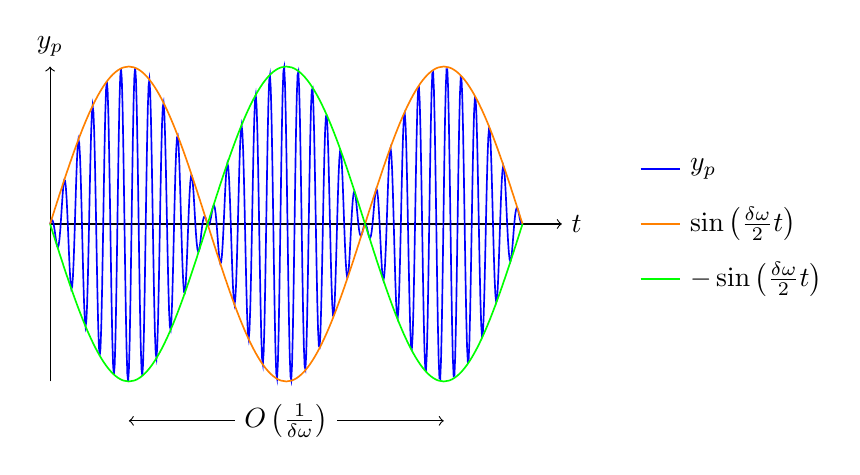
\begin{tikzpicture}
          \draw [->] (0, 0) -- (6.5, 0) node [right] {$t$};
          \draw [->] (0, -2) -- (0, 2) node [above] {$y_p$};
      
          \draw [semithick, blue, domain=0:6,samples=600] plot(\x, {2 * cos(2000 * \x) * sin (90 * \x)});
          \draw [semithick, orange] (0, 0) sin (1, 2) cos (2, 0) sin (3, -2) cos (4, 0) sin (5, 2) cos (6, 0);
          \draw [semithick, green] (0, 0) sin (1, -2) cos (2, 0) sin (3, 2) cos (4, 0) sin (5, -2) cos (6, 0);
      
          \draw [semithick, blue] (7.5, 0.7) -- (8, 0.7) node [black, right] {$y_p$};
          \draw [semithick, orange] (7.5, 0) -- (8, 0) node [black, right] {$\sin\left(\frac{\delta \omega}{2} t\right)$};
          \draw [semithick, green] (7.5, -0.7) -- (8, -0.7) node [black, right] {$-\sin\left(\frac{\delta \omega}{2} t\right)$};
      
          \draw [<->] (1, -2.5) -- (5, -2.5) node [pos=0.5,fill=white] {$O\left(\frac{1}{\delta \omega}\right)$};
        \end{tikzpicture}
      \end{center}
      Let $ \delta \omega\to 0 $, we get 
      \[
          \lim_{\delta \omega \to 0} \sin \left( \frac{\delta \omega}{2}t \right) \approx \frac{\delta \omega}{2}t
      ,\]
      and thus 
      \[
          \lim_{\delta \omega \to 0} y_p = -\frac{-t}{2\omega_0}\cos \omega_0 t
      .\]
      This represents a linear growth in amplitude. Note that $y_p$ takes form of complementary functions times an independent variable.
      \subsubsection{Impulses and point forces}
      Consider a system that experiences a sudden force. e.g., Consider a car driving over a speedbump. Suppose at time $T$ the car is above the bump, and at $T-\epsilon, T+\epsilon$ the car drives on and off the bump respectively. Consider $ \epsilon\to 0 $: force becomes a sudden impulse.
      \begin{center}
        \begin{tikzpicture}
          \draw [->] (-3, 0) -- (3.25, 0) node [right] {$t$};
          \draw [->, use as bounding box] (0, 0) node [below] {$T$} -- (0, 2.3) node [above] {force};
          \draw [semithick, orange, domain=-2.5:2.5, samples = 100] plot (\x, { 1.6 * exp( - 4 * \x * \x)});
        \end{tikzpicture}
      \end{center}
      Take $y$ as the disposition wrt $t$, the equation is 
      \begin{equation}
          M \ddot{y} = F(t)-ky-L \dot{y}
      \end{equation}
      Integrate this from $T-\epsilon$ to $T+\epsilon$:
      \[
          \begin{aligned}
            &\lim_{\epsilon \to 0} \int_{T-\epsilon}^{T+\epsilon} M \ddot{y} \,\mathrm{d}t = \lim_{\epsilon \to 0} \int_{T-\epsilon}^{T+\epsilon} F(t)-ky-L \dot{y} \,\mathrm{d}t\\
            \Longleftrightarrow & \lim_{\epsilon \to 0} M\left[ \dot{y} \right]_{T-\epsilon}^{T+\epsilon} = \lim_{\epsilon \to 0} \left\{ \int_{T-\epsilon}^{T+\epsilon} F(t) \,\mathrm{d}t - k \int_{T-\epsilon}^{T+\epsilon} y \,\mathrm{d}t - L\left[ y \right]_{T-\epsilon}^{T+\epsilon}\right\}\\
            \Longrightarrow & \lim_{\epsilon \to 0} M\left[ \dot{y} \right]_{T-\epsilon}^{T+\epsilon} = \lim_{\epsilon \to 0} \int_{T-\epsilon}^{T+\epsilon} F(t) \,\mathrm{d}t,
          \end{aligned}
      \]
      given that $y$ is finite and continuous.

      Define \textit{impulse} $I$ as 
      \[
          I =\lim_{\epsilon \to 0} \int_{T-\epsilon}^{T+\epsilon} F(t) \,\mathrm{d}t
      ,\]
      hence it becomes 
      \[
          I = \lim_{\epsilon \to 0} M\left[ \dot{y} \right]_{T-\epsilon}^{T+\epsilon}
      .\]
      Velocity $ \dot{y} $ experiences a sudden change(discontinuous) which depends on integral of force $ F(t) $.

      \subsubsection{Dirac delta function}\footnote{Lecture 16}
      Consider a family of functions $ D(t,\epsilon) $ such that 
      \begin{enumerate}
          \item $ \lim_{\epsilon \to 0} D(t,\epsilon)=0\  \forall t\neq 0 $,
          \item $\displaystyle \int_{-\infty}^{\infty} D(t,\epsilon) \,\mathrm{d}t =1$.
      \end{enumerate}
      \begin{example}
          $\displaystyle D(t,\epsilon)=\frac{1}{\epsilon\sqrt{\pi}}e^{-t^2/\epsilon^2} $. Note that
          \[
              \int_{-\infty}^{\infty} D(t,\epsilon) \,\mathrm{d}t=1
          .\]
          See sheet 1.
          \begin{center}
            \begin{tikzpicture}
              \draw [->] (-3, 0) -- (3.25, 0) node [right] {$t$};
              \draw [->, use as bounding box] (0, 0) -- (0, 4) node [above] {$D$};
          
              \draw [semithick, blue, domain=-3:3, samples = 100] plot (\x, { 1.6 * exp( - \x * \x)});
              \draw [semithick, orange, domain=-3:3, samples = 100] plot (\x, { 3.2 * exp( - 4 * \x * \x)});
          
              \draw [blue, semithick] (3.5, 2.25) -- (4, 2.25) node [right, black] {$\varepsilon = 1$};
              \draw [orange, semithick] (3.5, 1.75) -- (4, 1.75) node [right, black] {$\varepsilon = 0.5$};
            \end{tikzpicture}
          \end{center}
      \end{example}
      \begin{definition}
        Define \textit{Dirac delta function} as 
        \[
            \delta(x)=\lim_{\epsilon \to 0} D(x,\epsilon)
        .\]
      \end{definition}
      Properties of $ \delta(x) $:
      \begin{enumerate}
          \item $ \forall x\neq 0, \delta(x)=0 $.
          \item $\displaystyle \int_{-\infty }^{\infty } \delta(x) \,\mathrm{d}x=1$.
          \item (Sampling property) For continuous function $g(x)$, 
          \[
              \int_{-\infty}^{\infty} g(x)\delta(x) \,\mathrm{d}x = g(0)\int_{-\infty}^{\infty}  \delta(x)\,\mathrm{d}x = g(0)
          .\]
          More generally,
          \begin{equation}\label{eq:generalised sampling property}
            \int_{a}^{b} g(x)\delta(x-x_0) \,\mathrm{d}x = \begin{cases}
                g(x_0) &\text{if $ x_0\in [a,b] $.}\\
                0 &\text{otherwise.}\\
                \end{cases} 
          \end{equation}
      \end{enumerate}
      \begin{definition}
        We can define \textbf{Heaviside step function} from Dirac delta function $H(x)$ by 
        \begin{equation}\label{eq:heaviside step func}
            H(x)=\int_{-\infty}^{x} \delta(t) \,\mathrm{d}t.
        \end{equation}
      \end{definition}
      From FTC, $ H'=\delta(x) $.

      Properties of $H(x)$:
      \begin{enumerate}
          \item $H(x)=0$ for $x<0$.
          \item $H(x)=1$ for $x>0$.
          \item $ H(0) $ is undefined.
      \end{enumerate}
      \begin{center}
        \begin{tikzpicture}
          \draw [->] (-3, 0) -- (3, 0) node [right] {$x$};
          \draw [->] (0, 0) -- (0, 3) node [above] {$H(x)$};
    
          \draw [blue, semithick] (-3, 0) -- (0, 0);
          \draw [blue, semithick] (0, 2) node [left] {1} -- (3, 2);
        \end{tikzpicture}
      \end{center}
      \begin{definition}
          Define \textbf{Ramp function} as 
          \[
              r(x)=\int_{-\infty}^{x} H(t) \,\mathrm{d}t
          .\]
      \end{definition}      \begin{center}
        \begin{tikzpicture}
          \draw [->] (-3, 0) -- (3, 0) node [right] {$x$};
          \draw [->] (0, 0) -- (0, 3) node [above] {$r(x)$};
    
          \draw [blue, semithick] (-3, 0) -- (0, 0);
          \draw [blue, semithick, domain = 0:2.5] plot (\x, {\x});
        \end{tikzpicture}
      \end{center}
      Note that function get "smoother" as we integrate.
      \subsubsection{Delta function forcing}
      Consider
      \begin{equation}\label{eq:16.5}
        y''+p(x)y'+q(x)y=\delta(x).
      \end{equation}
      Note that highest order derivative "inherits" discontinuity from forcing.

      Since $\delta(x)=0$ for $x\neq 0$, 
      \[
          y''+py'+q=0, \quad \text{for }x< 0 \text{ and }x>0
      .\]
      $y(x)$ satisfies \textit{jump conditions}: 
      \begin{enumerate}
          \item $y(x)$ is continuous at $x=0$.
          \[
              \lim_{\epsilon \to 0} [y]_{x=-\epsilon}^{x=\epsilon}=0
          .\]
          \item $y'(x)$ has a jump of 1 at $x=0$. Integrate \ref{eq:16.5} in a small window around $x=0$:
          \[
              \lim_{\epsilon \to 0} \int_{-\epsilon}^{\epsilon} (16.5) \,\mathrm{d}x \Longrightarrow \lim_{\epsilon \to 0} [y']_{-\epsilon}^{\epsilon} = 1
          .\]
      \end{enumerate}
      Method for solution: Solve \ref{eq:16.5} for $ x<0 $ and $x>0$. This yields 4 unknown constants, so use 2 jump conditions and 2 initial conditions.
      \begin{example}
          Consider $ y''-y=3\delta(x-\frac{\pi}{2}) $. Set intial conditions to be $ y=0 $ at $ x=0,\pi $.

          For $ 0<x< \frac{\pi}{2} $, we have $ y''-y=0 \Rightarrow y=Ae^x+Be^{-x} $ or $ y= A \sinh x+B \cosh x $. $ y=0 $ at $x=0$, so $ y=A \sinh x $.

          Note that the equation is invariant $ x\to \pi-x $. By symmetry, for $ \frac{\pi}{2} $, $ y=C \sinh (\pi-x) $.

          Use the second jump condition:
          \[
              \begin{aligned}
                &\lim_{\epsilon \to 0} \int_{\frac{\pi}{2}-\epsilon}^{\frac{\pi}{2}+\epsilon} y''-y \,\mathrm{d}x = \lim_{\epsilon \to 0} [y']_{\frac{\pi}{2}-\epsilon}^{\frac{\pi}{2}+\epsilon} = 3\\
                \Longrightarrow & -C \cosh \frac{\pi}{2}-A \cosh \frac{\pi}{2}=3.
              \end{aligned}
          \]
          Use the first jump condition:
          \[
              \begin{aligned}
                &\lim_{\epsilon \to 0} [y]_{\frac{\pi}{2}-\epsilon}^{\frac{\pi}{2}+\epsilon}, \text{ shorthand notation } [y]^{\frac{\pi}{2}+}_{\frac{\pi}{2}-}=0\\
                \Longrightarrow & A \sinh \frac{\pi}{2}=C \sinh \frac{\pi}{2}\\
                \Longrightarrow & A=C=\frac{-3}{2\cosh \frac{\pi}{2}}.
              \end{aligned}
          \]
          Hence 
          \[
              y= \begin{cases}
              -\frac{3}{2}\frac{\sinh x}{\cosh \frac{\pi}{2}} &\text{if $ 0\le x<\frac{\pi}{2} $.}\\
              -\frac{3}{2}\frac{\sinh (\pi -x)}{\cosh \frac{\pi}{2}}&\text{if $ \frac{\pi}{2}<x\le \pi $}\\
              \end{cases} 
          .\]
          \begin{center}
            \begin{tikzpicture}
              \draw [->] (0, 0) -- (7, 0) node [right] {$x$};
          
              \draw [->] (0, 0) -- (0, -3.5) node [below] {$y$};
          
              \draw [semithick, blue, domain=0:1.5708] plot ({2 * \x}, {-1.3 * sinh (\x)});
              \draw [semithick, blue, domain=1.5708:3.14159] plot ({2 * \x}, {-1.3 * sinh (pi - \x)});
            \end{tikzpicture}
          \end{center}
      \end{example}
      \subsubsection{Heaviside step function forcing}
      Consider 
      \begin{equation}\label{eq:16.7}
        y''+p(x)y'+q(x)y=H(x-x_0).
      \end{equation}
      $y(x)$ satisfies
      \begin{equation}\label{eq:16.8}
        \begin{cases}
            y''+py'+qy=0 &\text{for }x<x_0,\\
            y''+py'+qy=1&\text{for }x>x_0.\\
          \end{cases}
      \end{equation}
      Evaluate \ref{eq:16.7} on either side of $x_0$:
          \[
            [y'']_{x_0-}^{x_0+}+p(x_0)[y']_{x_0-}^{x_0+}+q(x_0)[y]_{x_0-}^{x_0+}=1.
          \]
          If $ y'' \sim H \Rightarrow y' \sim r(x) \Rightarrow y\sim \int r(x) $, so $y',y$ are both continuous.

      The jump conditions here are 
      \begin{enumerate}
          \item $ [y']_{x_0-}^{x_0+}=0 $,
          \item $ [y]_{x_0-}^{x_0+}=0 $.
      \end{enumerate}
      Use ICs and jump conditions to find constants in solving the solution to \ref{eq:16.8}.
      \subsection{Higher order discrete(difference) equations}\footnote{Lecture 17}
      General form for $m$th order linear discrete equation with constant coefficients is
      \begin{equation}\label{eq:17.1}
          a_my_{n+m}+a_{m-1}y_{n+m-1}+\cdots+a_1y_{n+1}+a_0y_n=f_n.\footnote{Exploit same principles used to solve higher order ODEs.}
      \end{equation}
      \subsubsection{Eigenfunction}
      Consider a difference operator $D[y_n]=y_{n+1}$. It has eigenfunction $ y_n=k^n $, where $k$ is constant. This works since 
      \[
          D[k^n]=k^{n+1}=k\cdot k^n= ky_n
      .\]
      \subsubsection{Linearity}
      \ref{eq:17.1} is \textit{linear} in $y$. Hence we can write the solution in a sum of complementary function and a particular solution:
      \[
          y_n=y_n^{(c)}+y_n^{(p)}
      .\]
      \begin{example}
          Consider
          \[
              a_2y_{n+2}+a_1y_{n+1}+a_0y_n=f_n
          .\]
          We firstly solve the homogeneous equation 
          \[
            a_2y_{n+2}+a_1y_{n+1}+a_0y_n=0
          .\]
          Try $y_n=k^n$: 
          \[
              a_2k^2+a_1k+a_0=0
          ,\]
          which gives two solutions $k_1,k_2$. Therefore 
        \[
            y_n^{(c)}=\begin{cases}
            Ak_1^n+Bk_2^n &\text{ if }k_1\neq k_2,\\
            k^n(A+Bn) &\text{ if }k_1=k_2=k.\\
            \end{cases} 
        \]
      \end{example}
      \subsubsection{Particular integral}
      \begin{center}
        \begin{tabular}{cc}
        \toprule
        Form of $f_n$ & Form of $y_n^{(p)}$ \\ \midrule
        $ k^n $ & $ Ak^n $ if $ k\neq k_1,k_2 $ \\
        $ k_1^n, k_2^n $ & $ Ank_1^n+B_nk_2^n $ \\
        $ n^p $ & $ An^p+Bn^{p-1}+\cdots+Cn+D$ \\ \bottomrule
        \end{tabular}
    \end{center}
    \subsubsection{Fibonacci Sequence}
    General form is $ F_n=F_{n-1}+F_{n-2} $, and $ F_0=F_1=1 $. Standard for is 
    \[
        y_{n+2}-y_{n+1}-y_n=0
    .\]
    Try $y=k^n$:
    \[
        k^2-k-1=0 \Longleftrightarrow k_{1,2}=\frac{1\pm \sqrt{5}}{2}
    .\]
    We get 
    \[
        k_1=\phi\approx 1.618\dots,\quad k_2=-\frac{1}{\phi}
    .\]
    Since $k_1\neq k_2$, we have $ F_n=Ak_1^{n}+Bk_2^n $. Plugging in ICs gives 
    \[
        F_n = \frac{k_1^{n+1}-k_2^{n+1}}{\sqrt{5}} = \frac{1}{\sqrt{5}}\left( \phi^{n+1}-\left( -\frac{1}{\phi} \right)^{n+1} \right)
    .\]
    Also 
    \[
        \lim_{n \to \infty} \frac{F_{n+1}}{F_n} = \lim_{n \to \infty} \frac{\phi^{n+2}-(-1/\phi)^{n+2}}{\phi^{n+1}-(-1/\phi)^{n+1}}=\phi
    .\]
    \subsection{Series solutions for higher order ODEs}
    \subsubsection{Method of Frobenius}
    Series solutions applied to linear, homogeneous 2nd order ODEs. General form is 
    \begin{equation}\label{eq:17.2}
        p(x)y''+q(x)y'+r(x)y=0.
    \end{equation}
    seek power series expansion about $x=x_0$.
    
    \textbf{Firstly} classify $x=x_0$.
    \begin{definition}
        $x=x_0$ is an \textit{ordinary point} if Taylor series of $ q/p $ and $ r/p $ converge in some region around $x_0$. i.e., $ q/p, r/p $ are \textit{analytic}.

        Otherwise, $x=x_0$ is a \textit{singular point}.
    \end{definition} 
    \begin{definition}
        If $x=x_0$ is a singular point, but \ref{eq:17.2} can be written as 
        \[
            P(x)(x-x_0)^2y''+Q(x)(x-x_0)+R(x)y=0
        ,\]
        and $Q/P$ and $R/P$ are analytic, then $x=x_0$ is a \textit{regular singular point}.

        Otherwise, $x=x_0$ is an \textit{irregular} singular point.
    \end{definition}
    \begin{remark}
        $\displaystyle \frac{Q}{P}=(x-x_0)\frac{q}{p}, \frac{R}{P}=(x-x_0)^2\frac{r}{p}$. 
    \end{remark}
    \begin{example}
        \begin{enumerate}
            \item $ (1-x^2)y''-2xy'+2y=0 $. We have 
            \[
                \frac{q}{p}=\frac{-2x}{1-x^2}, x=\pm 1\text{ are singular points}
            .\]
            However, 
            \[
                \frac{Q}{P} = (x-1)\frac{q}{p}=\frac{2x}{1+x}
            ,\]
            so $1$ is a regular singular point. Similarly $-1$ is also a regular singular point.
            \item $ y'' \sin x + y' \cos x+2y=0 $. We have 
            \[
                \frac{q}{p}=\frac{\cos x}{\sin x}, \frac{r}{p}=\frac{2}{\sin x}
            .\]
            $ x=n\pi, n\in \mathbb{Z} $ are regular singular points.
            \item $ (1+\sqrt{x})y''-2xy'+2y=0 $.
            \[
                \frac{q}{p}=\frac{-2x}{1+\sqrt{x}}
            .\]
            Here $x=0$ is an irregular singular point.
            \bluecomment{Note: Second derivative is undefined.}
        \end{enumerate}
    \end{example}
    \begin{theorem}[Fuch]\label{thm:Fuch}\footnote{Lecture 18}
       \begin{enumerate}
           \item If $x_0$ is ordinary, then there are two linearly independent solutions of the form
           \[
               y=\sum_{n=0}^{\infty} a_n (x-x_0)^n
           ,\]
           convergent in some regions around $x_0$.
           \item If $x_0$ is a regular singular point, then there is \textit{at least one} solution of the form 
           \[
               y=\sum_{n=0}^{\infty}a_n(x-x_0)^{n+\sigma}
           ,\]
           where $ \sigma\in \mathbb{R} $ and $a_0\neq 0$.
       \end{enumerate} 
    \end{theorem}
    \begin{example}
        Consider 
        \[
            (1-x^2)y''+2xy'+2y=0\tag{$*$}
        .\]
        We find series solutions about $x=0$. Firstly divide $(1-x^2)$:
        \[
            y''-\frac{2x}{(1-x^2)}y'+\frac{2}{1-x^2}y=0
        .\]
        Hence $x=0$ is ordinary and we can plug in the form in 1.:
        \[
            y=\sum_{n=0}^{\infty}a_n x^n, y'=\sum_{n=1}^{\infty} na_nx^{n-1}, y''=\sum_{n=2}^{\infty }n(n-1)a_nx^{n-2}
        .\]
        \[
            \begin{aligned}
                x^2 \times (*) &\Longrightarrow (1-x^2)x^2y''-2x^2xy'+2x^2y=0\\
                &\Longleftrightarrow \sum_{n=2}^{\infty}a_nn(n-1)(1-x^2)x^n-2 \sum_{n=1}^{\infty}a_n(nx^2)x^n+2 \sum_{n=0}^{\infty}a_n x^2x^{n}=0.\\
            \end{aligned}
        \]
        Equate coefficients of $x^n$ for $n\ge 2$:
        \[
            a_n(n(n-1))-a_{n-2}(n-2)(n-3)-2a_{n-2}(n-2)+2a_{n-2}=0
        .\]
        This is a discrete equation for $a_n$. Write in standard form:
        \[
            n(n-1)a_n=(n^2-3n)a_{n-2} \Longleftrightarrow a_n = \frac{n-3}{n-1}a_{n-2}
        .\]
        Note that $a_0,a_1$ are not set by this recurrence relation and are arbitrary constants set by ICs. Note also that since $a_3=0$, $a_{2n+1}=0$ for $n\ge 1$. For $n$ even, 
        \[
            a_n=\frac{-1}{n-1}a_0
        .\]
        Therefore,
        \[
            y=a_1x+a_0\left( 1-x^2-\frac{x^4}{3}-\frac{x^6}{5}+\cdots \right)
        .\]
        From the fact that $ \ln (1\pm x) = \pm x-\frac{x^2}{2}\pm \frac{x^3}{3}-\cdots $ and that
        \[
            \begin{aligned}
                 \ln \left( \frac{1+x}{1-x} \right)&= \ln (1+x)-\ln (1-x)\\
                &= 2x+2\frac{x^3}{3}+\cdots,
            \end{aligned}
        \]
        we have 
        \[
            y=a_1 x+a_0\left( 1-\frac{x}{2}\ln \left( \frac{1+x}{1-x} \right) \right)
        .\]
        Note that behaviour near $x=\pm 1$ is singular and will be discussed  later.
    \end{example}
    \begin{example}
        Consider
        \[
            4xy''+2(1-x^2)y'-xy=0\tag{$**$}
        .\]
        We find series solutions about $x=0$. Clearly $0$ is a regular singular point. Hence try
        \[
            \begin{aligned}
                y&=\sum_{n=0}^{\infty}a_nx^{n+\sigma}, a_0\neq 0\\
                y'&= \sum_{n=0}^{\infty}a_n(n+\sigma)x^{n+\sigma-1}\\
                y''&=\sum_{n=0}^{\infty} a_n(n+\sigma)(n+\sigma-1)x^{n+\sigma-2}.
            \end{aligned}
        \]
        \[
            \begin{aligned}
                 x \times (**)&\Longrightarrow 4x^2y''+2(1-x^2)xy-x^2y=0\\
                &\Longleftrightarrow \sum_{n=0}^{\infty}a_nx^{n+\sigma}\left( 4(n+\sigma)(n+\sigma-1)+2(1-x^2)(x+\sigma)-x^2 \right)=0.
            \end{aligned}
        \]
        Equate coefficients of $x^{n+\sigma}$ for $n\ge 2$:
        \[
            a_n\left( 4(n+\sigma)(n+\sigma-1)+2(n+\sigma) \right)+a_{n-2}\left( -2(n-2+\sigma)-1 \right)=0
        .\]
        Which is 
        \[
            2(n+\sigma)(2n+2\sigma-1)a_n=(2n+2\sigma-3)a_{n-2}
        .\]
        To find $\sigma$, equate coefficients of lowest powers of $x$. Set $n=0$ and equate coefficients of $x^\sigma$:
        \[
            a_0(4\sigma(\sigma-1)+2\sigma)=0 \Longleftrightarrow 4\sigma(\sigma-1)+2\sigma=0 \Longleftrightarrow \sigma=0,\frac{1}{2}
        .\]
        If $ \sigma=0 $, equate coefficients of lowest powers of $x$. For $n=0$, the coefficient of $x_0$ is $a_0(0)=0$, so $a_0$ is arbitrary. For $n=1$, $ a_1(4 \cdot 1 \cdot 0)+a_1 \cdot 2 \cdot 1=0 \Leftrightarrow a_1=0 $. For $n\ge 2$ the recurrence relation applies so 
        \[
            a_n = \frac{2n-3}{2n(2n-1)}a_{n-2}
        .\]
        Note that for odd $n$ $a_n=0$. Therefore,
        \[
            y_1=a_0\left( 1+\frac{x^2}{4\cdot 3}+\frac{5x^4}{8\cdot 7\cdot 4\cdot 3}+\cdots \right)
        .\]

        If $\sigma=1/2$, then 
        \[
            2n(2n+1)b_n\footnote{use different lables to avoid confusion} = (2n-2)b_{n-2}
        .\]
        If $n=0$, 
        \[
            4\cdot \frac{1}{2}\cdot \left( -\frac{1}{2} \right)b_0+2\cdot \frac{1}{2}b_0=0 \Longleftrightarrow b_0 \text{ is arbitrary}
        .\]
        If $n=1$,
        \[
            \left( 4(1+\frac{1}{2})\cdot \frac{1}{2}+2(1+\frac{1}{2}) \right)b_1=0 \Longleftrightarrow b_1=0
        .\]
        Hence,
        \[
            y_2=b_0x^{\frac{1}{2}}\left( 1+\frac{x^2}{2\cdot 5}+\frac{3x^4}{2\cdot 5\cdot 4\cdot 9}+\cdots \right)
        .\]
        Here we found 2 linearly independent solutions.
    \end{example}
    \subsubsection{Special cases of the indicial equation}\footnote{Lecture 19.}
    Consider an expension about $x=x_0$, and let $ \sigma_1,\sigma_2 $ be the roots of initial indicial equation. The following proposition helps to determine the form of series solution. wlog, suppose $ \sigma_1\le \sigma_2 $.
    \begin{proposition}\label{prop:indicial equation}
        We have the following cases:
        \begin{enumerate}[label=\textbf{case} \arabic*]
            \item $ \sigma_1-\sigma_2\notin \mathbb{Z} $, then there are two linearly independent solutions of form 
            \[
                y=(x-x_0)^{\sigma_1}\sum_{n=0}^{\infty} a_n(x-x_0)^n+(x-x_0)^{\sigma_2}\sum_{n=0}^{\infty} b_n(x-x_0)^n.
            \]
            Note that $ y\sim (x-x_0)^{\sigma_1} $ as $ x\to 0 $.
            \item $ \sigma_1-\sigma_2\in \mathbb{Z} $. Then the solutions are of the form 
            \begin{align*}
                y_1&= (x-x_0)^{\sigma_2}\sum_{n=0}^{\infty} a_n(x-x_0)^n,\\
                y_2&=(x-x_0)^{\sigma_1}\sum_{n=0}^{\infty} b_n(x-x_0)^n+cy_1 \ln (x-x_0),
            \end{align*}
            where $c$ may or maynot be 0.
            \item $ \sigma_1=\sigma_2=\sigma $, here $c\neq 0$ so 
            \begin{align*}
                y_1&= (x-x_0)^{\sigma}\sum_{n=0}^{\infty} a_n(x-x_0)^n,\\
                y_2&=(x-x_0)^{\sigma}\sum_{n=0}^{\infty} b_n(x-x_0)^n+y_1 \ln (x-x_0).\footnote{Since any $c$ will just add a constant multiple in the combination $ \alpha y_1+\beta y_2 $, we can take $c=1$.}
            \end{align*}
        \end{enumerate}
    \end{proposition}\newpage
    \begin{example}
        Consider the equation
        \begin{equation}\label{eq:19.1}
            x^2y''-xy=0
        \end{equation}
        and find the series solutions at $x=0$. This is a regular singular point, so try
        \begin{align*}
            y&=\sum_{n=0}^{\infty}a_nx^{n+\sigma}, a_0\neq 0\\
            y'&= \sum_{n=0}^{\infty}a_n(n+\sigma)x^{n+\sigma-1}\\
            y''&=\sum_{n=0}^{\infty} a_n(n+\sigma)(n+\sigma-1)x^{n+\sigma-2}.
        \end{align*}
        We get 
        \[
            \sum_{n=0}^{\infty}a_nx^{n+\sigma}\left( (n+\sigma)(n+\sigma-1)-x \right)=0.
        \]
        Equate coefficients of $ x^{n+\sigma} $ for $n\ge 2$:
        \[
            a_n(n+\sigma)(n+\sigma-1)=a_{n-1}.
        \]
        The indicial equation is 
        \[
            \sigma(\sigma-1)a_0=0 \Longrightarrow \sigma=0,1,
        \]
        and it is an example of case 2.

        If $ \sigma=1 $, 
        \[
            a_n = \frac{a_{n-1}}{n(n+1)} = \frac{a_0}{(n+1)(n!)^2}.
        \]
        Hence one solution is 
        \[
            y_1 = (x-x_0) a_0\sum_{n=0}^{\infty} \frac{x^n}{(n+1)(n!)^2}.
        \]
        If $ \sigma=0 $, then 
        \[
            b_n = \frac{b_{n-1}}{n(n-1)} \text{ for }n\ge 2,\ b_0,b_1 \text{ arbitrary}.
        \]
        Therefore the sum is linearly dependent to $y_1$, and thus $c\neq 0$:\footnote{Actually, we can get this form via \textbf{reduction of order}, by setting $y_2=vy_1$ and solve the reduced DE.}
        \[
            y_2 = y_1 \ln x + b_0 + xb_1 + \sum_{n=2}^{\infty}\frac{x^n}{(n)((n-1!)^2}.
        \]
    \end{example}
    \begin{example}
        Review again $(1-x^2)y''+2xy'+2y=0,$ and seek a series solution expanded about $-1$. Let $z=1+x$, so it is equivalent to expand about $z=0$. We get 
        \[
            z(2-z)y''-2(z-1)y'+2y=0.
        \]
        Try $y=\sum_{n=0}^{\infty}a_nx^{n+\sigma}, a_0\neq 0$. Boring algebras give the indicial equation 
        \[
            2\sigma(\sigma-1)+2\sigma=0 \Longleftrightarrow \sigma=0.
        \]
        This is an example of case 3, and we need $ y_1\ln z $ term.
    \end{example}
    \section{Multivariable Functions and Applications}
    \subsection{Function of multiple independent variables}
    \subsubsection{Directional Derivative and Gradient Vector}\footnote{Lecture 20}
    Consider a function $f(x,y)$ and a small displacement vector $ \d \mathbf{s} $. Consider the rate of change of $f$ in direction $ \d \mathbf{s} $. Note that 
    \[
        \d f = \frac{\partial f}{\partial x}\d x+ \frac{\partial f}{\partial y}\d y = (\d x,\d y) \cdot \left( \frac{\partial f}{\partial x} ,\frac{\partial f}{\partial y}\right):=\d\mathbf{s} \cdot \nabla f,
    \]
    where $ \d \mathbf{s}=(\d x,\d y) $ and $ \nabla f = \left( \frac{\partial f}{\partial x} ,\frac{\partial f}{\partial y}\right) $ is the \textit{gradient vector} in cartesian coordinates. If we write $ \d \mathbf{s}=\d s \hat{\mathbf{s}} $, then we can rewrite the equation as 
    \[
        \d f = \d s (\hat{\mathbf{s}}\cdot \nabla f).
    \]
    \begin{definition}[Directional derivative]
        The \textit{directional derivative} of $f$ along $\hat{\mathbf{s}}$ is defined as 
        \[
            \frac{\mathrm{d}f}{\mathrm{d}s} = \hat{\mathbf{s}} \cdot \nabla f. 
        \]
    \end{definition}
    \begin{proposition}[Properties of gradient vector]\label{prop:properties of gradient vector}
        \begin{enumerate}
            \item The \textit{magnitude} of $\nabla f$ is the maximum rate of change of $f(x,y)$:
            \[
                \left| \nabla f \right| = \max_{\langle \hat{\mathbf{s}}, \nabla f \rangle } \frac{\mathrm{d}f}{\mathrm{d}s}. 
            \]
            \item The \textit{direction} of $\nabla f$ is the direction where $f$ \textit{increases} the most rapidly.
            \[
                \left| \frac{\mathrm{d}f}{\mathrm{d}s}  \right| = \left| \nabla f\right| \cos \langle \hat{\mathbf{s}},\nabla f \rangle.
            \]
            \item If $ \d \mathbf{s} $ and $\hat{\mathbf{s}}$ are parallel to contours of $f$, then 
            \[
                \frac{\mathrm{d}f}{\mathrm{d}s}=\hat{\mathbf{s}} \cdot \nabla f=0. 
            \]
            That is, $ \nabla f $ is perpendicular to contours of $f$ and $ |\nabla f| $ is the slope in the "uphill" direction.
        \end{enumerate}
    \end{proposition}
    \subsubsection{Stationary Points}
    In general, there is always at least one direction where $ \frac{\mathrm{d}f}{\mathrm{d}s}=0 $, parallel to the contours of $f$.
    \begin{definition}
        A \textit{stationary point} is a point at which 
        \[
            \forall \hat{\mathbf{s}}, \frac{\mathrm{d}f}{\mathrm{d}s}=0. 
        \]
    \end{definition}
    Since $ \frac{\mathrm{d}f}{\mathrm{d}s}=\hat{\mathbf{s}}\cdot \nabla f $, $ \nabla f=0 $ at stationary points.
    \subsubsection*{Types of stationary points}
    \begin{itemize}
        \item Local minimum,
        \item Local maximum,
        \item Saddle points:
        \begin{center}
            \begin{tikzpicture}
              \begin{axis}[hide axis, xtick=\empty, ytick=\empty]
                \addplot3 [mesh, draw=gray, samples = 11] {x^2 - y^2};
                \node [circ] at (axis cs:0, 0, 0) {};
              \end{axis}
            \end{tikzpicture}
          \end{center}
    \end{itemize}
    \begin{remark}
        Near min/max, the contours of $f$ are elliptical, and near saddle points the contours are hyperbolic. Contours of $f$ can only cross at saddle points.
    \end{remark}
    \subsubsection{Multivariable Taylor Series}
    Consider a point $\mathbf{s}_0$ and a small displacement $ \sigma\mathbf{s} = \delta s \hat{\mathbf{s}} $. The taylor series expansion in the direction of $\hat{\mathbf{s}}$ is 
    \[
        f(s_0+\delta s)=f(s_0)+\delta s \frac{\mathrm{d}f}{\mathrm{d}s}\Big|_{s_0}+\frac{1}{2}(\delta s)^2 \frac{\mathrm{d}^2f}{\mathrm{d}s^2}\Big|_{s_0}+\cdots  . 
    \]
    From definition of directional derivative, 
    \[
        \frac{\mathrm{d}}{\mathrm{d}s} = \hat{\mathbf{s}}\cdot \nabla. 
    \]
    Hence 
    \[
        \delta s \frac{\mathrm{d}}{\mathrm{d}s}=\delta\mathbf{s} \cdot \nabla . 
    \]
    Hence we can rewrite the expansion as 
    \[
        f(s_0+\delta s)=f(s_0)+\underbrace{\delta\mathbf{s} \cdot \nabla f}_{(1)}\Big|_{s_0}+\underbrace{\frac{1}{2}(\delta s)^2(\hat{\mathbf{s}}\cdot \nabla )^2 f}_{(2)}\Big|_{s_0}+\cdots .
    \]
    In cartesian coordinates,
    \[
        \mathbf{s}_0=(x_0,y_0), \delta\mathbf{s} = (\delta x,\delta y), x=x_0+\delta x, y=y_0+\delta y.
    \]
    Thus 
    \begin{align*}
        (1)&=\delta(x)\frac{\partial f}{\partial x}+\delta y \frac{\partial f}{\partial y}, \\
        (2)&= \frac{1}{2}\left( \delta x \frac{\partial }{\partial x}+\delta y \frac{\partial }{\partial y}   \right)^2 f\\
        &= \frac{1}{2}\left( \delta x^2 f_{xx}+\delta x\delta y (f_{xy}+f_{yx})+\delta_y f_{yy} \right)\\
        &= \frac{1}{2}(\delta x, \delta y) \begin{pmatrix}
            f_{xx}& f_{xy}\\
            f_{yx}& f_{yy}
        \end{pmatrix}
        \begin{pmatrix}
            \delta x\\ \delta y
        \end{pmatrix}
    \end{align*}
    \begin{definition}
        The \textit{Hessian matrix} is defined by 
        \[
            \mathbf{H} = \begin{pmatrix}
                f_{xx}& f_{xy}\\
            f_{yx}& f_{yy}
            \end{pmatrix} = \nabla (\nabla f).
        \]
    \end{definition}
    Therefore we have(in 2D cartesian coordinates)
    \begin{align*}
        f(x, y) &= f(x_0, y_0) + (x - x_0)f_x + (y - y_0)f_y \\
        &+ \frac{1}{2}[(x - x_0)^2 f_{xx} + 2(x - x_0)(y - y_0)f_{xy} + (y - y_0)^2 f_{yy}]
      \end{align*}
      and in general 
      \[
        f(\mathbf{x}) = f(\mathbf{x}_0 ) + \delta \mathbf{x}\cdot\nabla f(\mathbf{x}_0) + \frac{1}{2}\delta \mathbf{x}\cdot \nabla \nabla f\Big|_{\mathbf{x}_0}\cdot \delta \mathbf{x}^{\top}+ \cdots .
      \]
      \subsubsection{Classifying Stationary Points}
      Since $ \nabla f= \mathbf{0} $ defines a stationary point, the Taylor series about s.p. $ \mathbf{x}=\mathbf{x}_s $ is 
      \[
          f(\mathbf{x})\approx f(\mathbf{x}_s)+\frac{1}{2}\delta\mathbf{x} \mathbf{H}\Big|_{\mathbf{x}_s}\cdot \delta\mathbf{x}^{\top}.
      \]
      The nature of s.p. depends on $H$.

      Consider a function in $n$-dimensional space 
      \[
          f=f(x_1,\dots,x_n).
      \]
      We have
      \[
          \mathbf{H} = \begin{pmatrix}
              f_{x_1x_1}& \cdots & f_{x_1x_n}\\
              \vdots & \ddots & \vdots \\
              f_{x_nx_1}& \cdots & f_{x_nx_n}
          \end{pmatrix}.
      \]
      If $f_{x_ix_j}$ are defined for all $i,j$. Note that $f_{x_ix_j}=f_{x_jx_i}$. Hence $\mathbf{H}$ is symmetric and can be diagonalised wrt its principal axes.
      \[
          \delta\mathbf{x} \mathbf{H} \delta\mathbf{x}^{\top} = (\delta x_1,\dots,\delta x_n) \begin{pmatrix}
              \lambda_1&\cdots&0\\
              \vdots &\ddots &\vdots \\
              0& \cdots & \lambda_n
          \end{pmatrix}\begin{pmatrix}
              \delta x_1\\\vdots \\\delta x_n
          \end{pmatrix},
      \]
      where $ \lambda_i $ are eigenvalues of $\mathbf{H}$ and $ \delta x_i $ is the displacement along principal axes. Hence 
      \[
        \delta\mathbf{x} \mathbf{H} \delta\mathbf{x}^{\top} = \lambda_i\delta x_i^2.\quad (\text{summation convention})
      \]
      \begin{definition}[Signature of $\mathbf{H}$]
          The \textit{signatrue} of $\mathbf{H}$ is the pattern of signs of its subdeterminants.
      \end{definition}
      For example, for $f(x_1,\dots,x_n)$, the pattern of signs is the signs of 
      \[
          \underbrace{|f_{x_1x_1}|}_{|\mathbf{H}_1|}, \underbrace{\begin{vmatrix}
              f_{x_1x_1}&f_{x_1x_2}\\
              f_{x_2x_1}&f_{x_2x_2}
          \end{vmatrix}}_{|\mathbf{H}_2|}, \dots,\underbrace{\begin{vmatrix}
            f_{x_1x_1}& \cdots & f_{x_1x_n}\\
            \vdots & \ddots & \vdots \\
            f_{x_nx_1}& \cdots & f_{x_nx_n}
          \end{vmatrix}}_{|\mathbf{H}|}.
      \]
      If $H$ is positive(negative) definite, then $\mathbf{H}_1,\mathbf{H}_2,\dots,\mathbf{H}_{n-1}$ are also positive(negative definite)(Sylvester's criterion). i.e., a min/max point in $n$-dimensional space is also a min/max point in any subspace including the point.
      \subsubsection*{Types of stationary points}
      \begin{enumerate}
          \item Minimum, if $\delta\mathbf{x} \mathbf{H} \delta\mathbf{x}^{\top}>0$ for all $ \delta\mathbf{x} $. This means that $ \forall i, \lambda_i>0 $, and thus it happens if $H$ is positive definite, signature is $+,+,+,\dots$.
          \item Maximum, $\delta\mathbf{x} \mathbf{H} \delta\mathbf{x}^{\top}<0$ for all $\delta\mathbf{x}$, $ \lambda_i<0 $ and $\mathbf{H}$ is negative definite, signature is $-,+,-,+,\dots$.
          \item Saddle, $\mathbf{H}$ is indefinite, signatrue is non of above.
      \end{enumerate}
      \begin{remark}
          If $|\mathbf{H}|=0$, then we need higher order Taylor series. 
      \end{remark}
      \subsubsection{Contours of $f$ near s.p.}
      Consider a coordinate system along principal axes of $\mathbf{H}$:
      \[
          \mathbf{H}=\begin{pmatrix}
              \lambda_1&0\\
              0&\lambda_2
          \end{pmatrix}.
      \]
      Let $ \delta\mathbf{x}= (\mathbf{x}-\mathbf{x}_s)=(\xi,\eta) $. In a small region near $\mathbf{x}_s$, contours of $f$ satisfy:
      \begin{align*}
        f&=\text{constant} \approx f(\mathbf{x}_s)+\frac{1}{2}\delta\mathbf{x} \mathbf{H}\Big|_{\mathbf{x}_s}\cdot \delta\mathbf{x}^{\top}\\
        & \Longrightarrow \lambda_1 \xi^2+\lambda_2 \eta^2 \approx \text{constant}.
      \end{align*}
      Near min/max, $ \lambda_1,\lambda_2 $ have the same sign, so the contours are elliptical. Near saddle points $ \lambda_1,\lambda_2 $ have opposite signs, so the contours are hyperbolic.
      \begin{example}
          Consider 
          \[
              f(x,y)=4x^3-12xy+y^2+10y+6.
          \]
          The stationary points are $(x,y)=(1,1), (5,25)$. $f_{xx}=24x, f_{xy}=-12, f_{yy}=2$.

          For $(1,1)$, the pattern is $+,-$, so it is a saddle point.

          For $(5,25)$, the pattern is $+,+$, so it is a minimum.
      \end{example}
      \subsection{Systems of linear ODEs}
      \subsubsection{Baiscs}
      Consider 2 functions $y_1(t),y_2(t)$ which satisfy 
      \begin{align*}
        \dot{y_1} &= a y_1+by_2+f_1(t)\\
        \dot{y_2}&= cy_1+dy_2+f_2(t).
      \end{align*}
      In vector form,
      \[
          \dot{\mathbf{Y}} = M\mathbf{Y}+\mathbf{F},
      \]
      where 
      \[
          \mathbf{Y} = \begin{pmatrix}
            y_1\\y_2
          \end{pmatrix},M=\begin{pmatrix}
              a&b\\
              c&d
          \end{pmatrix}, \mathbf{F} = \begin{pmatrix}
            f_1\\f_2
          \end{pmatrix}.
      \]
      Any $n$th order DE can be written as a system of $n$ first order ODEs. e.g., the standard form of a 2nd order ODE is $ \ddot{y}+a \dot{y}+by=f $. Let $y_1=y, y_2=\dot{y}=\dot{y_1}$. Then $ \mathbf{Y}^{\top}=(y,\dot{y}) $. Hence we can write 
      \begin{align*}
          \dot{y_1}&= y_2,\\
          \dot{y_2}&= -ay_2-by_1+f,
      \end{align*} 
      or
      \[
          \dot{\mathbf{Y}}=\begin{pmatrix}
              0&1\\
              -b&-a
          \end{pmatrix}\mathbf{Y}+\begin{pmatrix}
              0\\f
          \end{pmatrix}.
      \]
    \subsubsection{Matrix Methods}
    To solve a system of linear ODEs:
    \[
        \dot{\mathbf{Y}}=M\mathbf{Y}+\mathbf{F}\tag{$*$}
    \]
    \begin{enumerate}
        \item Write $ \mathbf{Y} = \mathbf{Y}_c+\mathbf{Y}_p $, where 
        \[
            \dot{\mathbf{Y}_c}=M\mathbf{Y}_c.
        \]
        \item Seek solutions of $ \mathbf{Y}_c = \mathbf{v} e^{\lambda t} $:
        \[
            (*) \Longrightarrow \lambda\mathbf{v} = M\mathbf{v}.
        \]
        Note that $ \lambda,\mathbf{v} $ are eigenvalues and eigenvectors of $M$.
        \item Find $ \mathbf{Y}_p $ based on form of $\mathbf{F}$. 
    \end{enumerate}
    \begin{example}
        Consider 
        \[
            \dot{\mathbf{Y}}-\begin{pmatrix}
                -4&24\\
                1&-2
            \end{pmatrix}\mathbf{Y} = \begin{pmatrix}
                4\\1
            \end{pmatrix}e^t.
        \]
        The eigenvectors and eigenvalues of the matrix is $ \lambda_1=2, \mathbf{v}_1^{\top} = (4,1), \lambda_2 =-8, \mathbf{v}_2^\top =(-6,1) $, so
        \[
            \mathbf{Y}_c = A\begin{pmatrix}
                4\\1
            \end{pmatrix}e^{2t}+B\begin{pmatrix}
                -6\\1
            \end{pmatrix}e^{-8t}.
        \]
        For particular integral, try 
        \[
            \mathbf{Y}_p = \begin{pmatrix}
                u_1\\u_2
            \end{pmatrix}e^{t},
        \]
        where $u_1,u_2$ are unknown. 
        \begin{align*}
            &\begin{pmatrix}
                u_1\\u_2
            \end{pmatrix}-\begin{pmatrix}
                -4&24\\
                1&-2
            \end{pmatrix}\begin{pmatrix}
                u_1\\u_2
            \end{pmatrix} = \begin{pmatrix}
                4\\1
            \end{pmatrix}\\
            \Longrightarrow & \begin{pmatrix}
                5&-24\\
                -1&3
            \end{pmatrix}\begin{pmatrix}
                u_1\\u_2
            \end{pmatrix} = \begin{pmatrix}
                4\\1
            \end{pmatrix}\\
            \Longrightarrow & \begin{pmatrix}
                u_1\\u_2
            \end{pmatrix}=\begin{pmatrix}
                -4\\-1
            \end{pmatrix}.
        \end{align*}
        Hence the solution is 
        \[
            \mathbf{Y} = A\begin{pmatrix}
                4\\1
            \end{pmatrix}e^{2t}+B\begin{pmatrix}
                -6\\1
            \end{pmatrix}e^{-8t}-\begin{pmatrix}
                4\\1
            \end{pmatrix}e^{t}.
        \]
    \end{example}
    \begin{remark}
        If the forcing term on RHS matches with $ \mathbf{Y}_c $, try $ \mathbf{Y}_p = \mathbf{u} t e^{\lambda t} $.
    \end{remark}
    From a linear system of $n$ first order ODEs, we can construct $n$ uncoupled $n$th order ODEs.
    \begin{example}
        From the last example,
        \begin{align*}
            \dot{y_1}&= -4y_1+24y_2+4e^t,\\
            \dot{y_2}&= y_1-2y_2+e^t.
        \end{align*}
        Differentiate the first equation:
        \begin{align*}
            &\ddot{y_1} = -4 \dot{y_1}+24 \dot{y_2}+4e^t\\
            \Longrightarrow & \ddot{y_1} = -4 \dot{y_1}+24y_1-48y_2+28e^t\\
            \Longrightarrow & \ddot{y_1} +6 \dot{y_1}-16y_1=36e^t.
        \end{align*}
        Then the solution can be computed as 
        \[
            y_1 = Ae^{2t}+Be^{-8}t+ 4e^{t}.
        \]
        This indeed matches with the previous result.
    \end{example}
    \subsubsection{Phase Portraits Revisited}
    For complementary function $ \dot{\mathbf{Y}_c}=M\mathbf{Y}_c $, we see from previous section that 
    \[
        \mathbf{Y}_c = A\mathbf{v}_1 e^{\lambda_1 t}+B\mathbf{v}_2 e^{\lambda_2 t}.
    \]
    We have 3 cases for phase portraits:
    \begin{enumerate}
        \item $ \lambda_1,\lambda_2\in \mathbb{R}, \lambda_1 \lambda_2<0 $. wlog let $ \lambda_1>0, \lambda_2<0 $. The phase portrait looks like 
        \begin{center}
            \begin{tikzpicture}
              \draw [->] (-4, 0) -- (4, 0) node [right] {$y_1$};
              \draw [->] (0, -1.7) -- (0, 1.7) node [above] {$y_2$};
        
              \draw [->-=0.785, -<-=0.215, blue, semithick] (-4, -1) -- (4, 1) node [right] {$\mathbf{v}_1$};
              \draw [->-=0.25, -<-=0.75, blue, semithick] (-4, 0.667) -- (4, -0.667) node [right] {$\mathbf{v}_2$};
        
              \draw [blue, semithick, ->- = 0.3, ->- = 0.7] (-4, 1) .. controls (0, 0.333) and (0, 0.35) .. (4, 1.3);
              \draw [blue, semithick, -<- = 0.3, -<- = 0.7] (-4, -1.3) .. controls (0, -0.3) and (0, -0.333) .. (4, -1);
        
              \draw [blue, semithick, ->- = 0.3, ->- = 0.7] (-4, 0.333) .. controls (-2, 0) and (-2, -0.3) .. (-4, -0.6);
              \draw [blue, semithick, ->- = 0.3, ->- = 0.7] (4, -0.333) .. controls (2, 0) and (2, 0.3) .. (4, 0.6);
            \end{tikzpicture}
          \end{center}
          $(0,0)$ is a saddle node.
          \item $ \lambda_1,\lambda_2\in \mathbb{R}, \lambda_1,\lambda_2>0 $. If $ \lambda_1,\lambda_2<0 $, wlog suppose $ |\mathbf{v}_1|>|\mathbf{v}_2| $.
          \begin{center}
            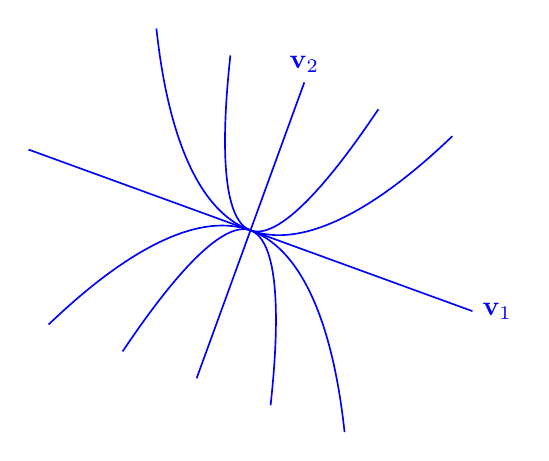
\begin{tikzpicture}[rotate=-20]
              \draw [blue, semithick] (-3, 0) -- (3, 0) node [right] {$\mathbf{v}_1$};
              \draw [blue, semithick] (0, -2) -- (0, 2) node [above] {$\mathbf{v}_2$};
      
              \draw [blue, semithick] (-2, 2) parabola bend (0, 0) (2, 2);
              \draw [blue, semithick] (-1, 2) parabola bend (0, 0) (1, 2);
              \draw [blue, semithick] (-2, -2) parabola bend (0, 0) (2, -2);
              \draw [blue, semithick] (-1, -2) parabola bend (0, 0) (1, -2);
            \end{tikzpicture}
          \end{center}
          If $ \lambda_1,\lambda_2>0 $, then it is called an \textit{unstable node}. The sketch is the same with arrow reversed.
          \item $ \lambda_1,\lambda_2 $ are complex conjugate. If $ \Re(\lambda_1,\lambda_2)<0 $
          \begin{center}
            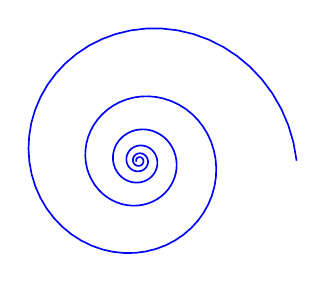
\begin{tikzpicture}
              \draw [blue, semithick, domain = 0:40,samples=300] plot ({2*exp(-\x/10)*cos(50*\x)}, {2*exp(-\x/10)*sin(50*\x)});
            \end{tikzpicture}
          \end{center}
          with arrow going in. This is a \textit{stable spiral}. If $ \Re(\lambda_1,\lambda_2)>0 $ then it is an \textit{unstable spiral} with arrow reversed. If $ \Re(\lambda_1,\lambda_2)=0 $, then we have cocentric ellipces called \textit{centre}. 
    \end{enumerate}
    \begin{remark}
        To find direction of rotation, we can evaluate system of equations at a given point to find sign of $ \dot{y_1},\dot{y_2} $.
    \end{remark}
    \subsubsection{Nonlinear Systems of ODEs}
    Consider an autonomous\footnote{$f,g$ are independent of time $t$} system of two nonlinear first order ODEs:
    \begin{align*}
        \dot{x}&= f(x,y),\\
        \dot{y}&= g(x,y).
    \end{align*}
    $f,g$ are nonlinear functions of $x,y$.
    \subsubsection*{Equilibrium(fixed) Points}
    Let $ (x_0,y_0) $ be a fixed point:
    \[
        \dot{x}|_{(x_0,y_0)} = \dot{y}|_{(x_0,y_0)}=0 \Rightarrow f(x_0,y_0)=g(x_0,y_0)=0.
    \]
    We solve this system for $(x_0,y_0)$.
    \subsubsection*{Stability of equilibrium points}
    Perturbation analysis: Consider a small displacement away from $(x_0,y_0)$:
    \[
        (x,y) = (x_0+\xi (t),y_0+\eta (t)).
    \]
    We have 
    \begin{align*}
        \dot{\xi} &= (x_0+\xi (t),y_0+\eta (t))\\
        &\approx f(x_0,y_0)+\xi f_x(x_0,y_0)+\eta f_y(x_0,y_0)
    \end{align*}
    and 
    \begin{align*}
        \dot{\eta}&=g(x_0+\xi,y_0+\eta)\\
        &\approx g(x_0,y_0)+\xi f_x(x_0,y_0)+\eta g_y(x_0,y_0)
    \end{align*}
    But $f(x_0,y_0)=g(x_0,y_0)=0$,  so 
    \[
        \begin{pmatrix}
            \dot{\xi}\\\dot{\eta}
        \end{pmatrix} = \begin{pmatrix}
            f_x&f_y\\
            g_x&g_y
        \end{pmatrix}\Big|_{(x_0,y_0)}\begin{pmatrix}
            \xi\\\eta
        \end{pmatrix}.
    \]
    This is a linear homogeneous system of ODEs. The eigenvalues of the matrix determine stability and behaviour. 
    \begin{example}[Phytoplankton and zooplankton: Predator-prey model or Lotka-Volterra equations]
        In a predator-prey system of phytoplanktons and zooplanktons, the populations of two species can be modelled as
        \begin{align*}
            \text{prey}\quad & \dot{x}=\alpha x- \beta xy=f(x,y),\\
            \text{predator}\quad & \dot{y} = \delta xy-\gamma y=g(x,y),
        \end{align*}
        where $ \alpha,\beta,\delta,\gamma>0 $.

        Consider the behaviour of the solution at a fixed point, where $ \dot{x}=\dot{y}=0 $.
        \begin{align*}
            \dot{x}=0 &\Longrightarrow x = 0 \lor y = \frac{\alpha}{\beta}\\
            \dot{y}=0& \Longrightarrow y = 0 \lor x = \frac{\gamma}{\delta}.
        \end{align*}
        Therefore the fixed points are $ (x_0,y_0)=(0,0), (\frac{\gamma}{\delta},\frac{\alpha}{\beta}) $. Note that 
        \[
            M=\begin{pmatrix}
                f_x&f_y\\
                g_x&g_y
            \end{pmatrix}=\begin{pmatrix}
                \alpha-\beta y&-\beta x\\
                \delta y&\delta x-\gamma
            \end{pmatrix}.
        \]
        At $(0,0)$, we have 
        \[
            \begin{pmatrix}
                \dot{\xi}\\\dot{\eta}
            \end{pmatrix} = \begin{pmatrix}
                \alpha&0\\
                0&-\gamma
            \end{pmatrix}\begin{pmatrix}
                \xi\\\eta
            \end{pmatrix}.
        \]
        The eigenvalues are $ \alpha>0,-\gamma<0 $, so it is a saddle node.

        At $ (\frac{\gamma}{\delta},\frac{\alpha}{\beta}) $, we have 
        \[
            \begin{pmatrix}
                \dot{\xi}\\\dot{\eta}
            \end{pmatrix} = \begin{pmatrix}
                0&-\frac{\gamma \beta}{\delta}\\
                \frac{\delta \alpha}{\beta}&0
            \end{pmatrix}\begin{pmatrix}
                \xi\\\eta
            \end{pmatrix}.
        \]
        By solving $ \lambda^2+\alpha \gamma=0 $, we get $ \lambda=\pm \sqrt{-\alpha\gamma}=\pm i \sqrt{\alpha\gamma} $. Hence $ \lambda $ are purely imaginary so it is a centre. For $x$, we have 
        \[
            \dot{\xi}=-\frac{\beta \gamma}{\delta}\eta.
        \]
        If $ \eta>0 $, $ \dot{\xi}<0 $, so the direction is counterclockwise.
    \end{example}
    \section{Partial Differential Equations}
    \begin{definition}
        A PDE is a DE with multiple independent variables.
    \end{definition}
    \subsection{First Order Wave Equation}
    Consider $ y(x,t) $ where 
    \[
        \frac{\partial y}{\partial t}-c \frac{\partial y}{\partial x}=0,\quad c = \text{constant}.  
    \]
    We solve by \textit{method of characteristics}, sample $y(x,t)$ along a path $x(t)$, so that the function becomes $ y(x(t),t) $. Note that 
    \[
        \frac{\mathrm{d}y}{\mathrm{d}t} = \frac{\partial y}{\partial t}+\frac{\partial y}{\partial x}\frac{\mathrm{d}x}{\mathrm{d}t}.    
    \]
    Compare with the standard form, if $ \frac{\mathrm{d}x}{\mathrm{d}t}=-c  $, then $ \frac{\mathrm{d}y}{\mathrm{d}t}=0  $. i.e., $y$ is constant along paths with $ x=x_0-ct, x_0\in \mathbb{R} $.
    \begin{center}
        \begin{tikzpicture}
          \draw [->] (-1, 0) -- (5, 0) node [right] {$x$};
          \draw [->] (0, -1) -- (0, 3) node [above] {$t$};
          \node [anchor = north east] at (0, 0) {$O$};
      
          \foreach \x in {1, 2, 3, 4, 5} {
            \draw [red] (\x- 0.5, 0) -- (\x - 1.5, 2.5);
          }
          \node [right] at (4, 1.5) {contours of $y$};
        \end{tikzpicture}
      \end{center}
      If $ y(x,0)=f(x) $, $ y = f(x_0) $ along characteristics. Hence the general solution is \footnote{Firstly consider a particular path, then consider all possible paths. This indeed gives the general solution.}
      \[
          y=f(x+ct).
      \]
      \begin{example}[Unforced wave equation]
          \[
              \frac{\partial y}{\partial t}-c \frac{\partial y}{\partial x}=0, \quad y(x,0)=x^2-3.  
          \]
          The solution is 
          \[
              y(x,t)=(x+ct)^2-3.
          \]
      \end{example}
      \begin{example}[Forced wave equation]
          \[
            \frac{\partial y}{\partial t}+5 \frac{\partial y}{\partial x}=e^{-t}, \quad y(x,0)=e^{-x^2}.
          \]
          Now 
          \[
              \frac{\mathrm{d}y}{\mathrm{d}t} = e^{-t} 
          \]
          along paths with $ \frac{\mathrm{d}x}{\mathrm{d}t} =5 $ or $ x=x_0+5t $. We have $ y=A-e^{-t} $ along paths. I.C.: at $t=0$, $x=x_0$ and $ y(x,0)=A-1=e^{-x_0^2} $. Hence 
          \[
              y(x,t)=1+e^{-x_0^2}-e^{-t} = 1+e^{-(x-5t)^2}-e^{-t}.
          \]
      \end{example}
      \subsection{Second Order Wave Equation}
      General form is 
      \[
          \frac{\partial^2 y}{\partial t^2}-c^2 \frac{\partial^2 y}{\partial x^2}=0.  
      \]
      Factor the differnetial operator:
      \[
          \left( \frac{\partial t}{\partial t}-c\frac{\partial }{\partial x}   \right)\left( \frac{\partial t}{\partial t}+c\frac{\partial }{\partial x}   \right)y=0.
      \]
      Note that operators commute, so 
      \[
         \frac{\partial t}{\partial t}-c\frac{\partial y }{\partial x}   =0\quad \text{or}\quad  \frac{\partial t}{\partial t}+c\frac{\partial y}{\partial x} =0.
      \]
      By comparison, we have 
      \[
          y=f(x+ct)\quad \text{or}\quad y=g(x-ct).
      \]
      Since the original equation is linear in $y$, general solution is 
      \[
          y = f(x+ct)+g(x-ct).\footnote{We need not add $A,B$ to make it a span, since $f,g$ are already general solutions.}
      \]
      \begin{example}
          Consider $ y_{tt}-c^2y_{xx}=0 $ subjected to $ y=\frac{1}{1+x^2}, y_t=0 $ at $t=0$. $ y\to 0 $ as $ x\to \pm \infty $. Solution is $ y=f(x+ct)+g(x-ct) $. Apply ICs:
          \begin{align*}
              &f(x)+g(x)=\frac{1}{1+x^2}\\
              &cf'(x)-cg'(x)=0\\
              \Longrightarrow & f'=g' \Longrightarrow f=g+A\\
              \Longrightarrow & 2g+A=\frac{1}{1+x^2} \Longrightarrow \begin{aligned}
                g(x)=\frac{1}{2}\left( \frac{1}{1+x^2}\right)-\frac{1}{2}A\\
                f(x)=\frac{1}{2}\left( \frac{1}{1+x^2}\right)+\frac{1}{2}A
              \end{aligned} 
          \end{align*}
          Hence the general solution is 
          \[
              y(x,t)=\frac{1}{2}\left( \underbrace{\frac{1}{1+(x+ct)^2}}_{\text{moves left}}+\underbrace{\frac{1}{1+(x-ct)^2}}_{\text{moves right}} \right), c>0.
          \]
      \end{example}
      \subsection{Diffusion Equation}
      \begin{example}
          Consider 
          \[
              \frac{\partial y}{\partial t} = \kappa \frac{\partial^2 y}{\partial x^2}  
          \]
          subjected to $ y(x,0)=\delta(x) $, the dirac delta function, and $ y\to 0, x\to \infty $. Define $ \eta=\frac{x^2}{4\kappa t} $, the \textit{similarity variable}.\footnote{Motivated by dimensional analysis: $\eta$ is dimensionless.}

          Seek solutions of form
          \[
              y=t^{-\alpha}f(\eta).
          \]
          $\alpha,f$ are to be determined. Note that $ y_t=-\alpha t^{-\alpha-1}f(\eta)+t^{-\alpha}f_{\eta}\eta_t, y_x=t^{-\alpha}f_{\eta}\eta_x, y_{xx}=t^{-\alpha}f_{\eta \eta}(\eta_x)^2+t^{-\alpha}f_{\eta}\eta_{xx}$. Then the original equation becomes 
          \[
              -\frac{\alpha}{t}f+f_{\eta}\eta_t=\kappa(f_{\eta \eta}(\eta_x)^2+f_\eta \eta_{xx}).
          \]
          Now 
          \[
              \eta_t = \frac{-x^2}{4\kappa t^2} = \frac{-\eta}{t}, \eta_x = \frac{1x}{2\kappa t}, (\eta_x)^2 = \frac{x^2}{4\kappa^2 t^2}= \frac{\eta}{\kappa t}, \eta_{xx}=\frac{1}{2\kappa t}.
          \]
          Hence it becomes 
          \[
              \alpha f+f'\eta+f''\eta+\frac{f'}{2}=0 \Longrightarrow \eta \frac{\mathrm{d}}{\mathrm{d}\eta}\left( f+f' \right) +\frac{1}{2}(f'+2\alpha f)=0.
          \]
          Thus we have turned the equation into an ODE.\footnote{$ \alpha $ is arbitrary at this stage.} Set $ \alpha=1/2 $, then 
          \[
            \eta \frac{\mathrm{d}}{\mathrm{d}\eta}\left( f+f' \right) +\frac{1}{2}(f+f')=0 \Longrightarrow \eta \frac{\mathrm{d}F}{\mathrm{d}\eta} +\frac{1}{2}F=0.(f+f'=F)
          \]
          One solution is $ F=0 \Rightarrow f+f'=0 \Rightarrow f=Ae^{-\eta} $. Recall that $ y=t^{-\alpha}f(\eta) $, so 
          \[
              y=A t^{-1/2}e^{-x^2/4\kappa t}.
          \]
          From ICs, recall that 
          \[
              \delta(x)=\lim_{\epsilon \to 0} \frac{1}{\epsilon\sqrt{\pi}}e^{-t^2/\epsilon^2}
          \]
        Let $ \epsilon^2=4 \kappa t $, then $ t\to 0 \Leftrightarrow \epsilon\to 0 $. Then 
        \[
            \delta(x)=\lim_{t \to 0} \frac{1}{\sqrt{4\pi \kappa}}t^{-1/2}e^{-x^2/4\kappa t} \Longrightarrow A=\frac{1}{\sqrt{4\pi \kappa}}.
        \]
        Therefore 
        \[
            y(x,t)=\frac{1}{\sqrt{4\pi \kappa}}t^{-1/2}e^{-x^2/4\kappa t}.
        \]
        This indeed matches with the second IC.
      \end{example}
\end{document}